%% abtex2-modelo-trabalho-academico.tex, v-1.9.6 laurocesar
%% Copyright 2012-2016 by abnTeX2 group at http://www.abntex.net.br/
%%
%% This work may be distributed and/or modified under the
%% conditions of the LaTeX Project Public License, either version 1.3
%% of this license or (at your option) any later version.
%% The latest version of this license is in
%%   http://www.latex-project.org/lppl.txt
%% and version 1.3 or later is part of all distributions of LaTeX
%% version 2005/12/01 or later.
%%
%% This work has the L PPL maintenance status `maintained'.
%%
%% The Current Maintainer of this work is the abnTeX2 team, led
%% by Lauro César Araujo. Further information are available on
%% http://www.abntex.net.br/
%%
%% This work consists of the files abntex2-modelo-trabalho-academico.tex,
%% abntex2-modelo-include-comandos and abntex2-modelo-references.bib
% ------------------------------------------------------------------------
% ------------------------------------------------------------------------
% abnTeX2: Modelo de Trabalho Academico (tese de doutorado, dissertacao de
% mestrado e trabalhos monograficos em geral) em conformidade com
% ABNT NBR 14724:2011: Informacao e documentacao - Trabalhos academicos -
% Apresentacao
% ------------------------------------------------------------------------
% ------------------------------------------------------------------------
% Personalização para o modelo Udesc 2020 7. ed. revisada e modificada
% MANUAL_2020_09_07_1599489825065_12510.pdf
% Autor: Felipe Joel Zimann (felipezimann@hotmail.com)
% Data: 02/12/2020 v1.0
% Data: 13/02/2021 v1.0.1 alterado tamanho numeração da página para 10pt
% ------------------------------------------------------------------------
% ------------------------------------------------------------------------

\documentclass[
	12pt,					% tamanho da fonte
	openright,				% capítulos começam em pág ímpar (insere página vazia caso preciso)
	oneside,				% para impressão em recto e verso (twoside). Oposto a (oneside)
	a4paper,				% tamanho do papel.
	chapter=TITLE,			% títulos de capítulos convertidos em letras maiúsculas
	section=TITLE,			% títulos de seções convertidos em letras maiúsculas
	sumario=abnt-6027-2012,
	english,				% idioma adicional para hifenização
	brazil,					% o último idioma é o principal do documento
	fleqn,					% equações alinhadas a esquerda (UDESC/CCT)+
]{abntex2}
\usepackage{hyperref}

% ----------------------------------------------------------
% Pacotes básicos 
% ----------------------------------------------------------
\usepackage{amsmath}							% Pacote matemático
\usepackage{amssymb}							% Pacote matemático
\usepackage{amsfonts}							% Pacote matemático
%\usepackage{lmodern}							% Usa a fonte Latin Modern		
\usepackage{mathptmx} 							% Usa a fonte Times New Roman	 (UDESC/CCT)
\usepackage[T1]{fontenc}						% Selecao de codigos de fonte.
\usepackage[utf8]{inputenc}						% Codificacao do documento (conversão automática dos acentos)
\usepackage{lastpage}							% Usado pela Ficha catalográfica
\usepackage{indentfirst}						% Indenta o primeiro parágrafo de cada seção.
\usepackage[dvipsnames,table]{xcolor}			% Controle das cores
\usepackage{graphicx}							% Inclusão de gráficos
\usepackage{microtype} 							% para melhorias de justificação
\usepackage{lipsum}								% para geração de dummy text
\usepackage[brazilian,hyperpageref]{backref}	% Paginas com as citações na bibl
\usepackage[alf,abnt-emphasize=bf,abnt-full-initials=yes]{abntex2cite}					% Citações padrão ABNT
%\usepackage[num]{abntex2cite}					% Citações padrão ABNT numérica
\usepackage{adjustbox}							% Pacote de ajuste de boxes
\usepackage{subcaption}							% Inclusão de Subfiguras e sublegendas		
\usepackage{enumitem}							% Personalização de listas
\usepackage{siunitx}							% Grandezas e unidades
\usepackage[section]{placeins}					% Manter as figuras delimitadas na respectiva seção com a opção [section]
\usepackage{multirow}							% Multi colunas nas tabelas
\usepackage{array,tabularx} 					% Pacotes de tabelas
\usepackage{booktabs}							% Pacote de tabela profissonal
\usepackage{rotating}							% Rotacionar figuras e tabelas
\usepackage{xfrac}								% Fazer frações n/d em linha
\usepackage{bm}									% Negrito em modo matemático
\usepackage{xstring}							% Manipulação de strings
\usepackage{pgfplots}							% Pacote de Gráficos
\usepackage{tikz}								% Pacote de Figuras
\usepackage[american, cuteinductors,smartlabels, fulldiode, siunitx, americanvoltages, oldvoltagedirection, smartlabels]{circuitikz}						% Pacote de circuitos elétricos
\usepackage{chemformula}						% Pacote para fórmulas químicas
\usepackage{chngcntr}							% Pacte usado para deixar numeração de equações sequencial (UDESC/CCT)
\counterwithout{equation}{chapter}
% fonte: https://latex.org/forum/viewtopic.php?t=15392

% Comando para deixar numeração das equações contínua (1), (2), (3)... ao invés de organizar por capítulos (1.1)(1.2)... (2.1)(2.2)
%\renewcommand{\theequation}{\arabic{equation}}

%\numberwithin{equation}{section}


% Cabecalho cabeçalho somente com numeração de página 10pt
\makepagestyle{PagNumReduzida}
\makeevenhead{PagNumReduzida}{\ABNTEXfontereduzida\thepage}{}{}
\makeoddhead{PagNumReduzida}{}{}{\ABNTEXfontereduzida\thepage}
%fonte: https://github.com/abntex/abntex2/wiki/HowToCustomizarCabecalhoRodape
%fonte: Manual memoir seção 7.3 pg. 111 pdf http://linorg.usp.br/CTAN/macros/latex/contrib/memoir/memman.pdf 

% Personalização das opções das listas
\setlist[itemize]{leftmargin=\parindent}

% Citação online --- MODIFICAR ---
\newcommand{\citeshort}[1]{\citeauthoronline{#1}~(\citeyear{#1})}

\newcommand{\me}[1]{Elaborado pelo autor (#1).}

% Configuração do pgfplots
\pgfplotsset{compat=newest} %compat=1.14
\pgfplotsset{plot coordinates/math parser=false} 
\newlength\figureheight 
\newlength\figurewidth 

% Libraries do TiKz
\usetikzlibrary{quotes,angles,arrows}
\usetikzlibrary{through,calc,math}
\usetikzlibrary{graphs,backgrounds,fit}
\usetikzlibrary{shapes,positioning,patterns,shadows}
\usetikzlibrary{decorations.pathreplacing}
\usetikzlibrary{shapes.geometric}
\usetikzlibrary{arrows.meta}
\usetikzlibrary{external}

%\tikzexternalize[]
%\tikzexternalenable
%\tikzexternalize
%\tikzexternaldisable
%\tikzset{external/force remake}
%\tikzexternalize[shell escape=-enable-write18]

% Configurações do CircuiTiKz
\ctikzset{bipoles/thickness=1}
%\ctikzset{bipoles/length=1.2cm}
\ctikzset{monopoles/ground/width/.initial=.2}
\ctikzset{bipoles/resistor/height=0.25}
\ctikzset{bipoles/resistor/width=0.6}
\ctikzset{bipoles/capacitor/height=0.5}
\ctikzset{bipoles/capacitor/width=0.15}
\ctikzset{bipoles/generic/height=0.25}
\ctikzset{bipoles/generic/width=0.6}
%\ctikzset{bipoles/capacitor polar/length=0.5}
%\ctikzset{bipoles/diode/height=.375}
%\ctikzset{bipoles/diode/width=.3}
%\ctikzset{tripoles/thyristor/height=.8}
%\ctikzset{tripoles/thyristor/width=1}
\ctikzset{bipoles/vsourcesin/height=.5}
\ctikzset{bipoles/vsourcesin/width=.5}
\ctikzset{bipoles/cvsourceam/height=.6}
\ctikzset{bipoles/cvsourceam/width=.6}
%\ctikzset{tripoles/european controlled voltage source/width=.4}

\tikzstyle{every node}=[font=\footnotesize]
\tikzstyle{every path}=[line width=0.25pt,line cap=round,line join=round]
%\tikzstyle{every path}=[line cap=round,line join=round]


% Definição de cores MATLAB
\definecolor{matlab_blue}{rgb}	{         0,    0.4470,    0.7410}
\definecolor{matlab_orange}{rgb}{    0.8500,    0.3250,    0.0980}
\definecolor{matlab_yellow}{rgb}{    0.9290,    0.6940,    0.1250}
\definecolor{matlab_violet}{rgb}{    0.4940,    0.1840,    0.5560}
\definecolor{matlab_green}{rgb}	{	 0.4660,    0.6740,    0.1880}
\definecolor{matlab_lblue}{rgb}	{    0.3010,    0.7450,    0.9330}
\definecolor{matlab_red}{rgb}	{    0.6350,    0.0780,    0.1840}

% Personalização das legendas
\usepackage[format = plain, %hang
			justification = centering,
			labelsep = endash,
			singlelinecheck = false,
			skip = 6pt,
			listformat = simple]{caption}	

% Personalização das unidades
\sisetup{output-decimal-marker = {,}}
\sisetup{exponent-product = \cdot, output-product = \cdot}
\sisetup{tight-spacing=true}
\sisetup{group-digits = false}

% Personalizações de tipo de colunas de tabelas
\newcolumntype{L}[1]{>{\raggedright\let\newline\\\arraybackslash\hspace{0pt}}m{#1}}
\newcolumntype{C}[1]{>{\centering\let\newline\\\arraybackslash\hspace{0pt}}m{#1}}
\newcolumntype{R}[1]{>{\raggedleft\let\newline\\\arraybackslash\hspace{0pt}}m{#1}}

% Personalizações de cores da UDESC
\definecolor{CapaAmareloUDESC}{RGB}{243,186,83}		% Especializacao
\definecolor{CapaVerdeUDESC}{RGB}{0,112,52}			% Mestrado
\definecolor{CapaVermelhoUDESC}{RGB}{171,35,21}		% Doutorado
\definecolor{CapaAzulUDESC}{RGB}{38,54,118} 		% Pós-Doutorado

% CONFIGURAÇÕES DE PACOTES
% Configurações do pacote backref
% Usado sem a opção hyperpageref de backref
\renewcommand{\backrefpagesname}{Citado na(s) página(s):~}
% Texto padrão antes do número das páginas
\renewcommand{\backref}{}
% Define os textos da citação
\renewcommand*{\backrefalt}[4]{
	\ifcase #1 %
	Nenhuma citação no texto.%
	\or
	Citado na página #2.%
	\else
	Citado #1 vezes nas páginas #2.%
	\fi}%

% alterando o aspecto da cor azul
%\definecolor{blue}{RGB}{41,5,195}

% informações do PDF
\makeatletter
\hypersetup{
	%pagebackref=true,
	pdftitle={\@title}, 
	pdfauthor={\@author},
	pdfsubject={\imprimirpreambulo},
	pdfcreator={LaTeX with abnTeX2},
	pdfkeywords={abnt}{latex}{abntex}{abntex2}{trabalho academico}, 
	colorlinks=true,       		% false: boxed links; true: colored links
	linkcolor=black,          	% color of internal links
	citecolor=black,        	% color of links to bibliography
	filecolor=black,      		% color of file links
	urlcolor=black,
	bookmarksdepth=4
}
\makeatother


\makeatletter
\newcommand{\includetikz}[1]{%
	\tikzsetnextfilename{#1}%
	\input{#1.tex}%
}
\makeatother

% ---
% Possibilita criação de Quadros e Lista de quadros.
% Ver https://github.com/abntex/abntex2/issues/176
%
\newcommand{\quadroname}{Quadro}
\newcommand{\listofquadrosname}{Lista de quadros}

\newfloat[chapter]{quadro}{loq}{\quadroname}
\newlistof{listofquadros}{loq}{\listofquadrosname}
\newlistentry{quadro}{loq}{0}

% configurações para atender às regras da ABNT
\setfloatadjustment{quadro}{\centering}
\counterwithout{quadro}{chapter}
\renewcommand{\cftquadroname}{\quadroname\space} 
\renewcommand*{\cftquadroaftersnum}{\hfill--\hfill}

\setfloatlocations{quadro}{hbtp} % Ver https://github.com/abntex/abntex2/issues/176
% ---


% Espaçamento depois do título
\setlength{\afterchapskip}{0.7\baselineskip}
% O tamanho do parágrafo é dado por:
\setlength{\parindent}{1.25cm}
% Controle do espaçamento entre um parágrafo e outro:
\setlength{\parskip}{0.0cm}  % tente também \onelineskip
%\SingleSpacing % Espaçamento simples 
\OnehalfSpacing % Espaçamento 1,5 (UDESC/CCT)
%\DoubleSpacing	% Espaçamento duplo

% ---
% Margens - NBR 14724/2011 - 5.1 Formato
% ---
\setlrmarginsandblock{3cm}{2cm}{*}
\setulmarginsandblock{3cm}{2cm}{*}
\checkandfixthelayout[fixed]
% ---


% To use externalize consider
%https://tex.stackexchange.com/questions/182783/tikzexternalize-not-compatible-with-miktex-2-9-abntex2-package
%Lauro Cesar digged into the problem until he came with a solution for me to test. And it Works!
%
%According to this link:
%
%The package calc changed the commands \setcounter and friends to be fragile. So you have to make them robust. The example below uses etoolbox with \robustify:
%
\usepackage{etoolbox}
\robustify\setcounter
\robustify\addtocounter
\robustify\setlength
\robustify\addtolength


%% How to silence memoir class warning against the use of caption package?
%% https://tex.stackexchange.com/questions/391993/how-to-silence-memoir-class-warning-against-the-use-of-caption-package
%\usepackage{silence}
%\WarningFilter*{memoir}{You are using the caption package with the memoir class}
%\WarningFilter*{Class memoir Warning}{You are using the caption package with the memoir class}

% --------------------------------------------------------
% INICIO DAS CUSTOMIZACOES PARA A UDESC
% --------------------------------------------------------

% --------------------------------------------------------
% Fontes padroes de part, chapter, section, subsection e subsubsection
% --------------------------------------------------------
% --- Chapter ---
\renewcommand{\ABNTEXchapterfont}{\fontseries{b}} %\bfseries
\renewcommand{\ABNTEXchapterfontsize}{\normalsize}
% --- Part ---
\renewcommand{\ABNTEXpartfont}{\ABNTEXchapterfont}
\renewcommand{\ABNTEXpartfontsize}{\LARGE}
% --- Section ---
\renewcommand{\ABNTEXsectionfont}{\normalfont}
\renewcommand{\ABNTEXsectionfontsize}{\normalsize}
% --- SubSection ---
\renewcommand{\ABNTEXsubsectionfont}{\fontseries{b}} %\bfseries
\renewcommand{\ABNTEXsubsectionfontsize}{\normalsize}
% --- SubSubSection ---
\renewcommand{\ABNTEXsubsubsectionfont}{\itshape}
\renewcommand{\ABNTEXsubsubsectionfontsize}{\normalsize}

\renewcommand{\ABNTEXsubsubsubsectionfont}{\normalfont}
\renewcommand{\ABNTEXsubsubsubsectionfontsize}{\normalsize}
% ---

% --------------------------------------------------------
% Fontes das entradas do sumario
% --------------------------------------------------------

\renewcommand{\cftpartfont}{\ABNTEXpartfont\selectfont}
\renewcommand{\cftpartpagefont}{\normalsize\selectfont}

\renewcommand{\cftchapterfont}{\ABNTEXchapterfont\selectfont}
\renewcommand{\cftchapterpagefont}{\normalsize\selectfont}

\renewcommand{\cftsectionfont}{\ABNTEXsectionfont\selectfont}
\renewcommand{\cftsectionpagefont}{\normalsize\selectfont}

\renewcommand{\cftsubsectionfont}{\ABNTEXsubsectionfont\selectfont}
\renewcommand{\cftsubsectionpagefont}{\normalsize\selectfont}

\renewcommand{\cftsubsubsectionfont}{\normalfont\itshape\selectfont}
\renewcommand{\cftsubsubsectionpagefont}{\normalsize\selectfont}

\renewcommand{\cftparagraphfont}{\normalfont\selectfont}
\renewcommand{\cftparagraphpagefont}{\normalsize\selectfont}

% --------------------------------------------------------
% Usando os pacotes hyperref, uppercase... 
% Para deixar a section do toc uppercase precisa de:
% --------------------------------------------------------
\usepackage{textcase}

\makeatletter

\let\oldcontentsline\contentsline
\def\contentsline#1#2{%
	\expandafter\ifx\csname l@#1\endcsname\l@section
	\expandafter\@firstoftwo
	\else
	\expandafter\@secondoftwo
	\fi
	{%
		\oldcontentsline{#1}{\MakeTextUppercase{#2}}%
	}{%
		\oldcontentsline{#1}{#2}%
	}%
}
\makeatother

% --------------------------------------------------------
% Renomenando as entradas de APÊNDICES E ANEXOS
% --------------------------------------------------------

\renewcommand{\apendicesname}{AP\^ENDICES}
\renewcommand{\anexosname}{ANEXOS}


% Manipulação de Strings
%\RequirePackage{xstring}

% Comando para inverter sobrenome e nome
\newcommand{\invertname}[1]{%
	\StrBehind{#1}{{}}, \StrBefore{#1}{{}}%
}%


% --------------------------------------------------------
% Alterando os estilos de Caption e Fonte
% --------------------------------------------------------
\makeatletter
% Define o comando \fonte que respeita as configurações de caption do memoir ou do caption
\renewcommand{\fonte}[2][\fontename]{%
	\M@gettitle{#2}%
	\memlegendinfo{#2}%
	\par
	\begingroup
	\@parboxrestore
	\if@minipage
	\@setminipage
	\fi
	\ABNTEXfontereduzida
	\configureseparator
	\captiondelim{\ABNTEXcaptionfontedelim}
	\@makecaption{#1}{\ignorespaces #2}\par
	\endgroup}


\captionstyle[\raggedright]{\raggedright}

\makeatother

\setlength{\cftbeforechapterskip}{0pt plus 0pt}
\renewcommand*{\insertchapterspace}{}

\newlength{\mylen}	% New length to use with spacing
\setlength{\mylen}{1pt}

\setlength{\cftbeforechapterskip}{\mylen}
\setlength{\cftbeforesectionskip}{\mylen}
\setlength{\cftbeforesubsectionskip}{\mylen}
\setlength{\cftbeforesubsubsectionskip}{\mylen}
\setlength{\cftbeforesubsubsubsectionskip}{\mylen}


% ---
% Ajuste das listas de abreviaturas e siglas ; e símbolos [Personalizada para UDESC com espaçamento 1,5]
% ---

% ---
% Redefinição da Lista de abreviaturas e siglas [Personalizada para UDESC com espaçamento 1,5]
\renewenvironment{siglas}{%
	\pretextualchapter{\listadesiglasname}
	\begin{symbols} 
		\setlength{\itemsep}{0pt}	% Ajuste para Espaçamento 1,5 (UDESC/CCT)
	}{% 
	\end{symbols}
	\cleardoublepage
}
% ---

% ---
% Redefinição da Lista de símbolos [Personalizada para UDESC com espaçamento 1,5]
\renewenvironment{simbolos}{%
	\pretextualchapter{\listadesimbolosname}
	\begin{symbols}
		\setlength{\itemsep}{0pt}	% Ajuste para Espaçamento 1,5 (UDESC/CCT)
	}{%
	\end{symbols}
	\cleardoublepage
}
% ---





% ---
% FIM DAS CUSTOMIZACOES PARA A  Universidade do Estado de Santa Catarina - UDESC/CCT
% ---





	% Incliu pacotes básicos

\usepackage{xargs}
\usepackage[colorinlistoftodos,prependcaption,textsize=footnotesize]{todonotes}
\newcommand{\com}[2][1=]{\todo[linecolor=green,backgroundcolor=green!25,bordercolor=green]{#2}}
\newcommand{\icom}[2][1=]{\todo[inline,linecolor=red,backgroundcolor=red!25,bordercolor=red]{#2}}
\reversemarginpar
\setlength{\marginparwidth}{2.5cm}

% -----------------------------------------------------------------
% Informações de dados para CAPA e FOLHA DE ROSTO
% -----------------------------------------------------------------
\titulo{Um Jogo para a Educação Financeira nas Escolas}%

\autor{Thiago Artur {}Schumann}%
\orientador{Prof. Dr. Marcelo {}de Souza}%
\instituicao{Universidade do Estado de Santa Catarina, Centro de Educação Superior do Alto Vale do Itajaí, Departamento de Engenharia de Software}%
\tipotrabalho{Trabalho de Conclusão de Curso (Graduação)}
\preambulo{Trabalho de Conclusão apresentado ao curso de Engenharia de Software do Centro de Educação Superior do Alto Vale do Itajaí (CEAVI), da Universidade do Estado de Santa Catarina (UDESC), como requisito parcial para a obtenção do grau de bacharel em Engenharia de Software.}
\local{Ibirama}%
\data{\the\year}%

% compila o indice
\makeindex

% -----------------------------------------------------------------
% Início do documento
% -----------------------------------------------------------------
\begin{document}

\selectlanguage{brazil}
\frenchspacing  % Retira espaço extra obsoleto entre as frases.

% -----------------------------------------------------------------
% ELEMENTOS PRÉ-TEXTUAIS
% -----------------------------------------------------------------
\pretextual

% ---
% Capa
% ---


% --------------------------------------------------------
% Capa Padrão
% --------------------------------------------------------
\renewcommand{\imprimircapa}{%
	\begin{capa}%
		\center

		{\fontseries{b}\selectfont\MakeTextUppercase{UNIVERSIDADE DO ESTADO DE SANTA CATARINA -- UDESC}}

		{\fontseries{b}\selectfont\MakeTextUppercase{CENTRO DE EDUCAÇÃO SUPERIOR DO ALTO VALE DO ITAJAÍ -- CEAVI  }}

		{\fontseries{b}\selectfont\MakeTextUppercase{ENGENHARIA DE SOFTWARE -- ESO  }}

		\vfill

		{\fontseries{b}\selectfont\MakeTextUppercase{\normalsize\imprimirautor}}

		\vfill
		\begin{center}
			{\fontseries{b}\selectfont\MakeTextUppercase{\imprimirtitulo}}
		\end{center}
		\vfill

		\vfill

		{\fontseries{b}\selectfont\MakeTextUppercase{\imprimirlocal}}
		\par
		{\fontseries{b}\selectfont \imprimirdata}
		\vspace*{1cm}
	\end{capa}
}



\imprimircapa				% Capa padrão

					% Elemento Obrigatório
% ---
% Folha de rosto
% ---








% --------------------------------------------------------
% folha de rosto 
% --------------------------------------------------------

\makeatletter

\renewcommand{\folhaderostocontent}{
	\begin{center}
		
		{\fontseries{b}\selectfont\MakeTextUppercase{\imprimirautor}}
		
		\vfill
		
		\begin{center}
			{\fontseries{b}\selectfont\MakeTextUppercase{\imprimirtitulo}}
		\end{center}
	
		\vspace*{1.5cm}

		\abntex@ifnotempty{\imprimirpreambulo}{%
			\hspace{.45\textwidth}
			{\begin{minipage}{.5\textwidth}
					\SingleSpacing
					\imprimirpreambulo\par
					\vspace*{4pt}
					{\imprimirorientadorRotulo~\imprimirorientador\par}
					\abntex@ifnotempty{\imprimircoorientador}{%
						{\imprimircoorientadorRotulo~\imprimircoorientador}%
					}%
			\end{minipage}}%
		}%
	
		
		\vfill
		
	{\fontseries{b}\selectfont\MakeTextUppercase{\imprimirlocal}}
	\par
	{\fontseries{b}\selectfont \imprimirdata}
	\vspace*{1cm}
	\end{center}
}


% (o * indica que haverá a ficha bibliográfica)
% ---
\imprimirfolhaderosto*
% ---


			% Elemento Obrigatório
% Caso não utilize a Ficha Catalográfica entre na folha de rosto e retire o * de dentro do arquivo FolhadeRosto
%
% ---
% Inserir a ficha bibliografica
% ---

% Isto é um exemplo de Ficha Catalográfica, ou ``Dados internacionais de
% catalogação-na-publicação''. Você pode utilizar este modelo como referência. 
% Porém, provavelmente a biblioteca da sua universidade lhe fornecerá um PDF
% com a ficha catalográfica definitiva após a defesa do trabalho. Quando estiver
% com o documento, salve-o como PDF no diretório do seu projeto e substitua todo
% o conteúdo de implementação deste arquivo pelo comando abaixo:



% \begin{fichacatalografica}
%     \includepdf{fig_ficha_catalografica.pdf}
% \end{fichacatalografica}


%	\setlength{\parindent}{0cm}
%	\setlength{\parskip}{0pt}
\begin{fichacatalografica}
	%\sffamily
	%\rmfamily
	\ttfamily \hbadness=10000
	\vspace*{\fill}					% Posição vertical
	\begin{center}					% Minipage Centralizado
		Para gerar a ficha catalográfica de teses e \\
		dissertações acessar o link:  \\
		https://www.udesc.br/bu/manuais/ficha

		\vspace*{8pt}

		%	\begin{minipage}[c]{8cm}
		%	\centering \sffamily
		%	 Ficha catalográfica elaborada pelo(a) autor(a), com auxílio do programa de geração automática da Biblioteca Setorial do CCT/UDESC
		%	\end{minipage}
		\fbox{\begin{minipage}[c]{12.5cm}		% Largura
				\flushright
				{\begin{minipage}[c]{10.5cm}		% Largura
						\vspace{1.25cm}
						%\footnotesize
						\setlength{\parindent}{1.5em}
						\noindent \invertname{\imprimirautor} \par
						\imprimirtitulo{ }/{ }\imprimirautor. -- \imprimirlocal, \imprimirdata .\par
						\pageref{LastPage} p. : il. ; 30 cm.\par
						\vspace{1.5em}
						\imprimirorientadorRotulo~\imprimirorientador.\par
						\imprimircoorientadorRotulo~\imprimircoorientador.\par
						\imprimirtipotrabalho~--~\imprimirinstituicao, \imprimirlocal, \imprimirdata.\par
						\vspace{1.5em}
						1. Palavra-chave.
						2. Palavra-chave.
						3. Palavra-chave.
						4. Palavra-chave.
						5. Palavra-chave.
						I. \invertname{\imprimirorientador}.
						II. \invertname{\imprimircoorientador}.
						III. \imprimirinstituicao.
						IV. Título. %
						\vspace{1.25cm}	%		
					\end{minipage}%
				}% 
			\end{minipage}}%

		\vspace*{0.5cm}

	\end{center}
\end{fichacatalografica}


%\begin{fichacatalografica}
%	\sffamily
%	\vspace*{\fill}					% Posição vertical
%	\begin{center}					% Minipage Centralizado
%	\fbox{\begin{minipage}[c][8cm]{13.5cm}		% Largura
%	\small
%	\imprimirautor
%	%Sobrenome, Nome do autor
%	
%	\hspace{0.5cm} \imprimirtitulo  / \imprimirautor. --
%	\imprimirlocal, \imprimirdata-
%	
%	\hspace{0.5cm} \pageref{LastPage} p. : il. (algumas color.) ; 30 cm.\\
%	
%	\hspace{0.5cm} \imprimirorientadorRotulo~\imprimirorientador\\
%	
%	\hspace{0.5cm}
%	\parbox[t]{\textwidth}{\imprimirtipotrabalho~--~\imprimirinstituicao,
%	\imprimirdata.}\\
%	
%	\hspace{0.5cm}
%		1. Palavra-chave1.
%		2. Palavra-chave2.
%		3. Palavra-chave3.
% 		4. Palavra-chave4.
%		5. Palavra-chave5.
%		I. Orientador.
%		II. Universidade xxx.
%		III. Faculdade de xxx.
%		IV. Título 			
%	\end{minipage}}
%	\end{center}
%\end{fichacatalografica}
% ---

	% Elemento Obrigatório (Verso da Folha)
%
% ---
% Inserir errata
% ---
\begin{errata}
	Elemento opcional.

	Exemplo:

	\vspace{\onelineskip}

	SOBRENOME, Prenome do Autor. Título de obra: subtítulo (se houver). Ano de depósito. Tipo do trabalho (grau e curso) - Vinculação acadêmica, local de apresentação/defesa, data.

	\begin{table}[htb]
		\center
		\begin{tabular}{|p{2.4cm}|p{2cm}|p{3cm}|p{3cm}|}
			\hline
			\textbf{Folha} & \textbf{Linha} & \textbf{Onde se lê} & \textbf{Leia-se} \\
			\hline
			1              & 10             & auto-conclavo       & autoconclavo     \\
			\hline
		\end{tabular}
	\end{table}

\end{errata}
% ---				% Elemento Opcional

% ---
% Inserir folha de aprovação
% ---

% Isto é um exemplo de Folha de aprovação, elemento obrigatório da NBR
% 14724/2011 (seção 4.2.1.3). Você pode utilizar este modelo até a aprovação
% do trabalho. Após isso, substitua todo o conteúdo deste arquivo por uma
% imagem da página assinada pela banca com o comando abaixo:
%
% \includepdf{folhadeaprovacao_final.pdf}
%
\begin{folhadeaprovacao}



	\begin{center}
		{\fontseries{b}\selectfont\MakeTextUppercase{\normalsize\imprimirautor}}
	\end{center}
	\vfill

	\vfill
	\begin{center}
		{\fontseries{b}\selectfont\MakeTextUppercase{\imprimirtitulo}}
	\end{center}
	\vfill


	\abntex@ifnotempty{\imprimirpreambulo}{%
		\hspace{.45\textwidth}
		{\begin{minipage}{.5\textwidth}
				\SingleSpacing
				\imprimirpreambulo\par
				\vspace*{4pt}
				{\imprimirorientadorRotulo~\imprimirorientador\par}
				\abntex@ifnotempty{\imprimircoorientador}{%
					{\imprimircoorientadorRotulo~\imprimircoorientador}%
				}%
			\end{minipage}}%
	}%


	\vfill

	\begin{center}

		{\fontseries{b}\selectfont BANCA EXAMINADORA: }
		\vspace*{1.75cm}

		Prof. Dr. Marcelo de Souza \par
		UDESC
	\end{center}

	{Membros:}

	\begin{center}
		\vspace*{1.25cm}
		Nome do Orientador e Titulação \par
		Nome da Instituição

		\vspace*{1.25cm}
		Nome do Orientador e Titulação \par
		Nome da Instituição

		\vspace*{1.25cm}
		Nome do Orientador e Titulação \par
		Nome da Instituição


	\end{center}

	\vspace*{\fill}
	\begin{center}
		{\imprimirlocal, 01 de maio de \imprimirdata}
	\end{center}
	\vspace*{0.25cm}
\end{folhadeaprovacao}
% ---




%\textbf{	{Orientador: \vspace{-16pt} }
%	\assinatura{\textbf{Prof. \imprimirorientador , Dr.} \\ Univ. XXX} 
%	{Coorientador: \vspace{-16pt}}   
%	\assinatura{\textbf{Prof. \imprimircoorientador , Dr.} \\ Univ. XXX}
%	
%	{Membros: \vspace{-16pt} } 
%	
%	% --- Exemplo de assinaturas em sequência ---       
%	\setlength{\ABNTEXsignwidth}{8.5cm}
%	
%	\assinatura{\textbf{Prof. Professor, Dr.} \\ Univ. XXX}
%	\assinatura{\textbf{Prof. Professor, Dr.} \\ Univ. XXX}
%	\assinatura{\textbf{Prof. Professor, Dr.} \\ Univ. XXX}
%	
%	% --- Exemplo de assinaturas lado a lado ---
%	\setlength{\ABNTEXsignwidth}{7.5cm}
%
%    \noindent\hfill\assinatura*{\textbf{Prof. Professor, Dr.} \\ Univ. XXX}%
%    \hfill%
%    \assinatura*{\textbf{Prof. Professor, Dr.} \\ Univ. XXX}%
%    \hfill
%    
%    \noindent\hfill\assinatura*{\textbf{Prof. Professor, Dr.} \\ Univ. XXX}%
%    \hfill%
%    \assinatura*{\textbf{Prof. Professor, Dr.} \\ Univ. XXX}%
%    \hfill}		% Elemento Obrigatório
%% ---
% Dedicatória
% ---
\begin{dedicatoria}
	\vspace*{\fill}
	%   \begin{flushright}
	%   \noindent
	%	Este trabalho é dedicado às crianças adultas que,\\
	%	quando pequenas, sonharam em se tornar cientistas. 
	%   \end{flushright}

	{%
		\noindent\hspace{.5\textwidth}
		{\begin{minipage}{.5\textwidth}
				\begin{flushleft}
					Aos estudantes da Universidade do Estado de Santa Catarina, pela inspiração de sempre!
				\end{flushleft}
			\end{minipage}}%
		\vspace*{3cm}
	}%

\end{dedicatoria}
% ---
			% Elemento Opcional
% ---
% Agradecimentos
% ---
\begin{agradecimentos}
Agradeço ao meu orientador por aceitar conduzir o meu trabalho de pesquisa.
A todos os meus professores do curso de da Universidade do Estado de Santa Catarina – Udesc pela excelência da qualidade técnica de cada um.

Aos meus pais que sempre estiveram ao meu lado me apoiando ao longo de toda a minha trajetória. Sou grato à minha família pelo apoio que sempre me deram durante toda a minha vida.

Como disse Snoop Dog: ``Eu quero me agradecer por acreditar em mim mesmo, quero me agradecer por todo esse trabalho duro. Quero me agradecer por não tirar folgas. Quero me agradecer por nunca desistir. Quero me agradecer por ser generoso e sempre dar mais do que recebo. Quero me agradecer por tentar sempre fazer mais o certo do que o errado. Quero me agradecer por ser eu mesmo o tempo inteiro''.

Deixo um agradecimento especial ao meu orientador pelo incentivo e pela dedicação do seu escasso tempo ao meu projeto de pesquisa.


\end{agradecimentos}
% ---		% Elemento Opcional
% ---
% Epígrafe
% ---
\begin{epigrafe}
	\vspace*{\fill}
	%	\begin{flushright}
	%		\textit{``Eu não falhei, encontrei 10 mil soluções que não davam certo.'' (EDISON, [19--])}
	%	\end{flushright}
	{%
		\noindent\hspace{.5\textwidth}
		{\begin{minipage}{.5\textwidth}
				\begin{flushright}
					``Eu não falhei, encontrei 10 mil soluções que não davam certo.'' (EDISON, [19--])
				\end{flushright}
			\end{minipage}}%
		\vspace*{3cm}
	}%
\end{epigrafe}
% ---				% Elemento Opcional
% ---
% RESUMOS
% ---

% resumo em português
\setlength{\absparsep}{18pt} % ajusta o espaçamento dos parágrafos do resumo
\begin{resumo}
Elemento obrigatório que contém a apresentação concisa dos pontos relevantes do trabalho, fornecendo uma visão rápida e clara do conteúdo e das conclusões do mesmo. A apresentação e a redação do resumo devem seguir os requisitos estipulados pela NBR 6028 (ABNT, 2003). Deve descrever de forma clara e sintética a natureza do trabalho, o objetivo, o método, os resultados e as conclusões, visando fornecer elementos para o leitor decidir sobre a consulta do trabalho no todo.

 \textbf{Palavras-chave}: Palavra 1. Palavra 2. Palavra 3. Palavra 4. Palavra 5.
\end{resumo}
				% Elemento Obrigatório
% ---
% Abstract
% ---

% resumo em inglês
\begin{resumo}[Abstract]
	\begin{otherlanguage*}{english}
		Elemento obrigatório para todos os trabalhos de conclusão de curso. Opcional para os demais trabalhos acadêmicos, inclusive para artigo científico. Constitui a versão do resumo em português para um idioma de divulgação internacional. Deve aparecer em página distinta e seguindo a mesma formatação do resumo em português.

		\textbf{Keywords}: Keyword 1. Keyword 2. Keyword 3. Keyword 4. Keyword 5.
	\end{otherlanguage*}
\end{resumo}
				% Elemento Obrigatório

% ---
% inserir lista de ilustrações
% ---
\pdfbookmark[0]{\listfigurename}{lof}
\listoffigures*
\cleardoublepage
% ---

% ---
% inserir lista de quadros
% ---
%\pdfbookmark[0]{\listofquadrosname}{loq}
%\listofquadros*
%\cleardoublepage
% ---


% ---
% inserir lista de tabelas
% ---
\pdfbookmark[0]{\listtablename}{lot}
\listoftables*
\cleardoublepage
% ---

% ---
% inserir lista de abreviaturas e siglas
% ---
\begin{siglas}
	\item[ABNT] Associação Brasileira de Normas Técnicas
	\item[BU] Biblioteca Universitária
	\item[IN] Instrução Normativa
	\item[NBR] Normas Técnicas Brasileiras
	\item[TCC] Trabalho de Conclusão de Curso
	\item[Udesc] Universidade do Estado de Santa Catarina
\end{siglas}
% ---

% ---
% inserir lista de símbolos
% ---


\begin{simbolos}
  \item[@] Arroba
  \item[\%] Porcento
  \item[$^\circ$C] Graus Celsius
  \item[Ca] Cálcio
\end{simbolos}

% ---
				% Elemento Opcional
% ---
% inserir o sumario
% ---
\pdfbookmark[0]{\contentsname}{toc}
\tableofcontents*
\cleardoublepage
% ---
				% Elemento Obrigatório

% -----------------------------------------------------------------
% ELEMENTOS TEXTUAIS
% -----------------------------------------------------------------
\textual

\pagestyle{PagNumReduzida}						% Comando para cabeçalho somente com numeração de página 10pt
\aliaspagestyle{chapter}{PagNumReduzida}		% Deixar numeração da primeira página com tamanho igual ao resto da numeração

\chapter{Introdução}

A educação financeira representa um eixo fundamental na formação do ser humano. Segundo a \cite{OECD}, as crianças de hoje têm acesso ao dinheiro e começam a usar serviços financeiros digitais desde cedo. Elas estão crescendo em um cenário financeiro que evolui rapidamente, o que significa mais oportunidades, mas também maior responsabilidade individual nas decisões relacionadas a finanças pessoais, quando comparado com gerações anteriores. É importante que as crianças entendam conceitos financeiros importantes e comecem a desenvolver atitudes e comportamentos financeiramente responsáveis desde cedo.

Neste cenário, crianças e adolescentes são frequentemente expostos a um vasto volume de informações e estímulos, muitos oriundos de intensas campanhas de marketing que procuram influenciar seus hábitos de consumo desde a tenra idade. Essas campanhas, muitas vezes sofisticadas, não só promovem o consumo, mas também podem distorcer a percepção entre necessidade e desejo, como discutido por \cite{Junger_Medeiros_Moura_Barrocal_Amaral_2019}. Esta exposição precoce aos conceitos de consumo pode predispor os jovens a padrões de consumo impulsivos.

A atuação do Governo Federal do Brasil, por meio da implementação da Estratégia Nacional de Educação Financeira (ENEF) e do Fórum Brasileiro de Educação Financeira (FBEF), estabelecidas respectivamente pelos Decretos nº~7.397/2010 e nº~10.393/2020 \cite{decreto_10939}, é de grande importância. Essas políticas visam incorporar a educação financeira ao currículo escolar desde os anos iniciais, proporcionando aos estudantes uma base robusta para o desenvolvimento de competências financeiras.

A implementação da educação financeira nas escolas produz efeitos positivos em toda a sociedade. Além do benefício direto aos estudantes, suas famílias também são impactadas positivamente. Segundo \cite{Frisancho2023Spillover}, isso é particularmente significativo para famílias em situações socioeconômicas desfavoráveis, onde a educação financeira pode ser um vetor de transformação. \cite{Ozkale2023Designing} complementa ao sugerir que a integração de tarefas matemáticas com conceitos financeiros desde cedo estabelece uma base sólida para a literacia financeira contínua.

Atualmente, os jogos educativos digitais têm se destacado como ferramentas eficazes para aumentar o engajamento e a retenção dos estudantes. \cite{lee2023} ressalta que a gamificação (ou ludificação), que incorpora elementos de jogos em ambientes educacionais, exerce um impacto positivo no engajamento e no aprendizado dos estudantes, especialmente em disciplinas como matemática. \cite{dahalan2023} também enfatiza que a gamificação pode aprimorar o desempenho acadêmico e a motivação dos estudantes.

Conforme destacado por \cite{masnan2016financial}, a educação financeira é essencial desde a infância, preparando as crianças para se tornarem consumidores e gestores competentes. A introdução desses conceitos nas escolas inicia o processo de capacitação das crianças para enfrentar futuros desafios financeiros, desenvolvendo habilidades, atitudes e conhecimentos essenciais sobre literacia financeira. Essas competências são ainda mais necessárias em vista das mudanças nos padrões de emprego e das elevadas taxas de desemprego em muitos países. Assim, o desenvolvimento de um programa de educação financeira eficaz, eficiente e viável torn


\section{Problema}

O ensino tradicional, uma abordagem comum nas escolas, enfrenta desafios em manter o engajamento e o interesse dos estudantes na era atual. Embora ainda tenha seu valor, a eficácia das aulas expositivas tem sido questionada. De acordo \cite{fortes2023aprendizagem}, a busca por métodos educacionais inovadores é cada vez mais relevante para enriquecer o processo de aprendizagem. A variedade de conteúdos e a complexidade das matérias às vezes não são suficientes para manter a atenção dos estudantes, tornando a inovação educacional uma necessidade.

A situação financeira da população brasileira destaca a urgência dessa inovação. Conforme dados recentes do \cite{SERASA_2023}, em janeiro de 2023, o número de brasileiros inadimplentes atingiu um recorde na série histórica, chegando a 70,1 milhões. Isso representa aproximadamente 35\% da população, que alcançou 203 milhões de habitantes segundo o \cite{IBGE_Censo_2022}. Essas estatísticas são alarmantes e reforçam a necessidade de uma educação financeira sólida desde os primeiros anos de vida. A inadimplência não é apenas um problema econômico, mas também social, e sua prevenção começa com a educação.

Nesse contexto, jogos digitais surgem como uma ferramenta educacional promissora. Para \cite{Cruz_Araujo_Andrye_Galvao_Madeira_2022}, eles têm o potencial de transformar a aprendizagem em uma experiência mais envolvente e interativa. Além de manter os estudantes interessados, os jogos estimulam a criatividade, a imaginação e incentivam a colaboração e o trabalho em equipe. No entanto, é essencial que a introdução de jogos no ambiente educacional seja feita de maneira ponderada. Os educadores devem avaliar cuidadosamente a adequação dos jogos à faixa etária e ao conteúdo programático, garantindo que eles complementem, e não substituam, o currículo tradicional.

Portanto, diante dos desafios apresentados, surge a proposta de desenvolver um jogo digital focado auxílio do ensino de conceitos de educação financeira para estudantes do Ensino Fundamental. O objetivo é utilizar essa ferramenta como um meio complementar para enriquecer o processo de ensino e aprendizagem, e preparar os estudantes para enfrentar os desafios financeiros da vida adulta.

\section{Objetivos}
Esta seção apresenta o objetivo geral e os objetivos específicos do presente trabalho.

\subsection{Objetivo Geral}
Auxiliar a aprendizagem de conceitos básicos de educação financeira de estudantes do Ensino Fundamental por meio d eum jogo educativo digital.

\subsection{Objetivos Específicos}
\begin{enumerate}[noitemsep,nosep,labelindent=\parindent,leftmargin=*,label={\alph*}) ]
	\item Examinar detalhadamente o conteúdo de educação financeira fornecido pela Estratégia Nacional da Educação Financeira (ENEF) para o 5º ano do Ensino Fundamental.
	\item Projetar e desenvolver um jogo sério, inspirado na primeira narrativa do material da ENEF.
	\item Realizar uma análise crítica comparativa entre o presente trabalho e os trabalhos correlatos na área de educação financeira e jogos educativos.
\end{enumerate}

\section{Justificativa}

A aprendizagem através de práticas lúdicas, que engloba atividades centradas em brincadeiras e jogos, tem sido reconhecida por sua capacidade intrínseca de engajar e enriquecer a formação do indivíduo \cite{Santos_Thayna_da_silva_2021}. Estas práticas não apenas cultivam habilidades cognitivas, mas também nutrem competências socioemocionais, como criatividade, empatia e capacidade de interação social. A natureza interativa e envolvente das atividades lúdicas é especialmente percebida no contexto educacional infantil, onde a atenção e o engajamento podem ser desafiadores de serem mantidos através de métodos pedagógicos tradicionais.

Dentro deste panorama, a proposta deste trabalho é aprimorar a experiência educacional ao digitalizar um jogo didático destinado ao 5º ano do Ensino Fundamental. A motivação por trás desta iniciativa é dupla. Primeiro, adaptar-se à crescente inclinação das crianças por interações digitais e, segundo, enriquecer o material pedagógico tornando-o mais interativo e visualmente atraente. A versão atual do jogo, predominantemente textual e com limitações visuais, corre o risco de não capturar plenamente o interesse dos estudantes. Portanto, através da digitalização e enriquecimento do jogo, almeja-se oferecer uma ferramenta pedagógica que seja ao mesmo tempo educativa e engajante.

Além disso, a eficácia da gamificação em promover a literacia financeira, conforme demonstrado por \cite{inchamnan2019gamification}, oferece um respaldo empírico para a abordagem deste projeto. A gamificação não apenas motiva através de recompensas e feedback positivo, mas também tem o potencial de influenciar comportamentos financeiros a longo prazo. Assim, a incorporação de elementos gamificados no jogo didático proposto visa não apenas aumentar o engajamento dos estudantes, mas também fornecer um meio eficaz de educação financeira alinhado com a Estratégia Nacional da Educação Financeira (ENEF).


\section{Metodologia}

Para alcançar os objetivos propostos neste trabalho, foi realizada a digitalização de um dos três jogos fornecidos para o 5º ano do Ensino Fundamental pela ENEF. Atualmente, esses jogos são apresentados em um formato de livro-jogo, o que pode dificultar a sua intuitividade. A digitalização envolve a identificação dos cenários e o mapeamento dos fluxos de caminhos possíveis. Isso permite que os jogadores façam escolhas que os direcionem por diferentes trajetórias, cada uma com suas respectivas consequências.

Antes de iniciar o desenvolvimento de um jogo sério, é crucial a incorporação de elementos de um \textit{Game Design Document} (GDD) ao projeto. O GDD constitui-se como um documento abrangente que detalha cada elemento do jogo, abarcando a narrativa, as mecânicas, o projeto de níveis, além dos recursos visuais e sonoros. Esse documento serve como um roteiro para o(s) desenvolvedor(es), assegurando que todos os participantes do projeto tenham uma compreensão uniforme e detalhada do mesmo. A implementação eficaz do GDD é vital para assegurar que o jogo não apenas seja bem desenvolvido, mas também atinja os objetivos pedagógicos propostos, conforme destacado por \cite{arifudin2022gdd}.

O jogo será estruturado em cenários distintos, cada um representando uma fase específica da narrativa. Diferentemente de jogos tradicionais de \textit{Role-Playing Game} (RPG), onde o jogador controla diretamente o movimento do personagem, o foco será nas escolhas que o jogador faz. Essas decisões influenciarão o percurso da narrativa, levando o personagem por diferentes caminhos e impactando o desfecho da história. Dependendo das escolhas feitas, o jogo pode ser concluído mais rapidamente, às vezes sem alcançar os objetivos principais. Para a implementação, utilizou-se o \textit{framework} RPG Maker MZ \cite{RPGMakerMZ}, que é especialmente adequado para a criação de RPGs. Esse \textit{framework} facilita a construção de mapas para cada cenário, contribuindo para uma experiência imersiva e interativa. Além disso, a compatibilidade do RPG Maker MZ com as plataformas \textit{web}, \textit{Windows} e \textit{MacOS} permite que o jogo seja acessível a um número maior de dispositivos e, consequentemente, de pessoas.

A fase de análise crítica deste trabalho envolveu uma comparação detalhada entre o jogo sério desenvolvido e os trabalhos correlatos no campo da educação financeira e gamificação educacional, sem aplicação direta com estudantes. Essa análise se baseou em critérios estabelecidos na literatura para proporcionar uma avaliação objetiva e abrangente, incluindo:

\begin{itemize}
	\item \textbf{Design Pedagógico}: Análise da estrutura educacional do jogo, incluindo os objetivos de aprendizagem, conteúdo, e estratégias pedagógicas empregadas.
	\item \textbf{Design de Jogo e Mecânicas}: Avaliação das mecânicas de jogo, narrativa, e como estes elementos apoiam os objetivos educacionais.
	\item \textbf{Usabilidade e Experiência do Usuário}: Análise da interface, facilidade de uso e acessibilidade do jogo.
	\item \textbf{Adequação ao Público-Alvo}: Verificação de se o jogo é apropriado para a faixa etária e contexto educacional a que se destina.
	\item \textbf{Comparação com a Literatura}: Análise de como o jogo se compara com outros trabalhos similares em termos de design, conteúdo, eficácia educacional e inovação.
	\item \textbf{Viabilidade e Sustentabilidade}: Discussão sobre a viabilidade de implementação do jogo em ambientes educacionais e sua sustentabilidade a longo prazo.
	\item \textbf{Relevância e Contribuição para a Área}: Avaliação da contribuição do jogo para o campo da educação financeira e gamificação.
\end{itemize}

\chapter{Fundamentação Teórica}
Este capítulo busca contextualizar os principais conceitos abordados no presente trabalho, tais como os materiais utilizados como base e também a tecnologia adotada no desenvolvimento do projeto. Ao final, são listados e discutidos alguns trabalhos correlatos.

\section{Estratégia Nacional de Educação Financeira}

\icom{As ideias desta seção precisam ser referenciadas. Referencie algum documento ou site da ENEF, e também o material didático que você está explorando.}

A Estratégia Nacional de Educação Financeira (ENEF) representa uma resposta proativa e estruturada às crescentes demandas de uma sociedade que enfrenta desafios financeiros complexos. Instituída com o objetivo de aprimorar a conscientização financeira da população brasileira, a ENEF busca não apenas promover a cidadania, mas também equipar os indivíduos com as ferramentas necessárias para tomar decisões financeiras informadas.

Essa estratégia abrange um amplo espectro de áreas de estudo, que vão desde os direitos e deveres básicos até tópicos mais complexos, como investimentos, previdência e planejamento financeiro. A inclusão de temas como poupança, crédito, seguros e consumo demonstra a abordagem abrangente adotada pela ENEF. Ao abordar temas tão variados, a ENEF reconhece e enfatiza que a educação financeira é um processo contínuo, que deve começar na infância e continuar ao longo da vida.

%\subsection{Material Didático}

A ENEF destaca-se por sua abordagem prática, evidenciada por sua ampla variedade de materiais didáticos. Foram elaborados 24 livros especificamente alinhados com a missão educacional da ENEF. Cada livro foi cuidadosamente desenvolvido para atender às necessidades de diferentes faixas etárias: 18 destinados ao Ensino Fundamental e os 6 restantes focados no Ensino Médio. Uma característica notável é a separação dos livros em materiais específicos para alunos e guias para professores, garantindo que o conteúdo seja adequadamente direcionado para cada público.

Os primeiros livros têm como objetivo familiarizar os alunos do Ensino Fundamental com conceitos fundamentais de cidadania. Através de situações cotidianas, como a organização de uma sala de aula ou a coordenação de eventos escolares, os alunos são introduzidos a princípios de planejamento e organização. Conforme avançam na série, são gradualmente expostos a temas financeiros mais sofisticados, desde o entendimento básico das contas domésticas até a compreensão da origem e da trajetória do dinheiro na sociedade.

Dentre os materiais didáticos, os chamados ``livros-jogo'' se destacam por suas narrativas envolventes. Ao invés de simplesmente transmitir informações, esses livros contam histórias que permitem aos alunos explorar cenários financeiros e entender as consequências de várias decisões. Esse enfoque narrativo é enriquecido por discussões em livros subsequentes, que oferecem \textit{insights} sobre o papel de diferentes instituições financeiras e seu impacto na sociedade.

Nos 5º e 6º livros da série ENEF, observa-se uma abordagem pedagógica inovadora e envolvente, que reflete a excelência e o comprometimento da ENEF em proporcionar uma educação financeira de qualidade. Estes volumes adotam um formato interativo de livro-jogo. Enquanto o jogo digital foca na jogabilidade, o livro-jogo se destaca por sua capacidade de envolver o leitor em uma narrativa rica, permitindo-lhe tomar decisões que influenciam os rumos da história.

\icom{Referencie todas as figuras (e outros elementos como tabelas) pelo seu label, dessa forma você não precisa se preocupar com a numeração. Fiz um exemplo na referência à Figura~\ref{fig:figure-1}.}

A Figura~\ref{fig:figure-1} ilustra um esquema que destaca alguns dos caminhos possíveis que a história pode seguir. Esse diagrama demonstra a complexidade e a diversidade de trajetórias que um jogador pode experimentar, refletindo diferentes escolhas financeiras e suas respectivas consequências\com{Os números indicam as páginas? Se sim, colocar esse comentário.}.

\begin{figure}[ht]
	\centering
	\caption{Esquema com alguns dos caminhos possíveis da primeiro jogo/história.}
	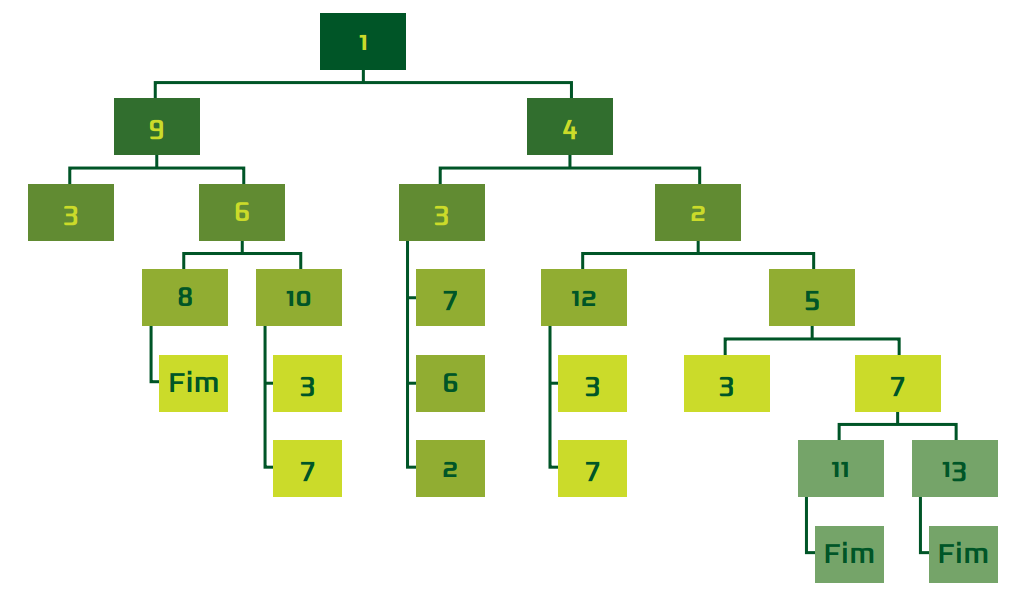
\includegraphics[scale=0.3]{Textuais/Pictures/Picture1.png}
	\fonte{\cite{Educacao_financeira_nas_escolas_professor}}\label{fig:figure-1}
\end{figure}

As Figuras 2 e 3\com{Atualizar} retratam momentos cruciais na narrativa do livro-jogo. Em cada figura, o leitor é introduzido a um cenário e, posteriormente, confrontado com duas ou três opções de ação. Cada escolha desencadeia diferentes desenvolvimentos na história, ilustrando as implicações de suas decisões no mundo financeiro.

\begin{figure}[ht]
	\centering
	\caption{Momento de decisão com duas possibilidades de caminhos.}
	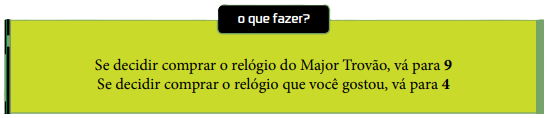
\includegraphics[scale=.85]{Textuais/Pictures/Picture2.png}
	\fonte{\cite{Educacao_financeira_nas_escolas}}\label{fig:figure-2}
\end{figure}

\begin{figure}[ht]
	\centering
	\caption{Momento de decisão com duas possibilidades de caminhos.}
	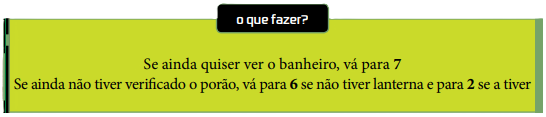
\includegraphics[scale=.85]{Textuais/Pictures/Picture3.png}
	\fonte{\cite{Educacao_financeira_nas_escolas}}\label{fig:figure-3}
\end{figure}

\newpage

Na continuação da série, principalmente nas fases finais do Ensino Fundamental, a ENEF aprofunda a abordagem, introduzindo conceitos mais avançados e específicos sobre o universo financeiro. Os alunos são expostos a uma variedade de instituições financeiras e suas respectivas funções. Por exemplo, ao aprender sobre bancos, os estudantes ganham experiência sobre operações bancárias, sistemas de crédito e a importância da gestão financeira. Quando o tema é agências de viagens ou hotéis, os alunos são introduzidos ao mundo das transações comerciais, tarifas, reservas e a economia do turismo. Essa abordagem detalhada serve para ampliar o horizonte dos alunos e prepará-los para interações financeiras mais complexas no futuro.

\section{RPG Maker MZ}

O RPG Maker MZ é uma plataforma robusta de desenvolvimento de jogos, especializada em jogos de interpretação de personagens (RPG). Essa ferramenta oferece uma ampla gama de recursos pré-construídos e interfaces intuitivas, possibilitando que desenvolvedores possam criar experiências interativas ricas e complexas \cite{RPGMakerMZ}.

\begin{figure}[ht]
	\centering
	\caption{Interface do RPG Maker MZ.}
	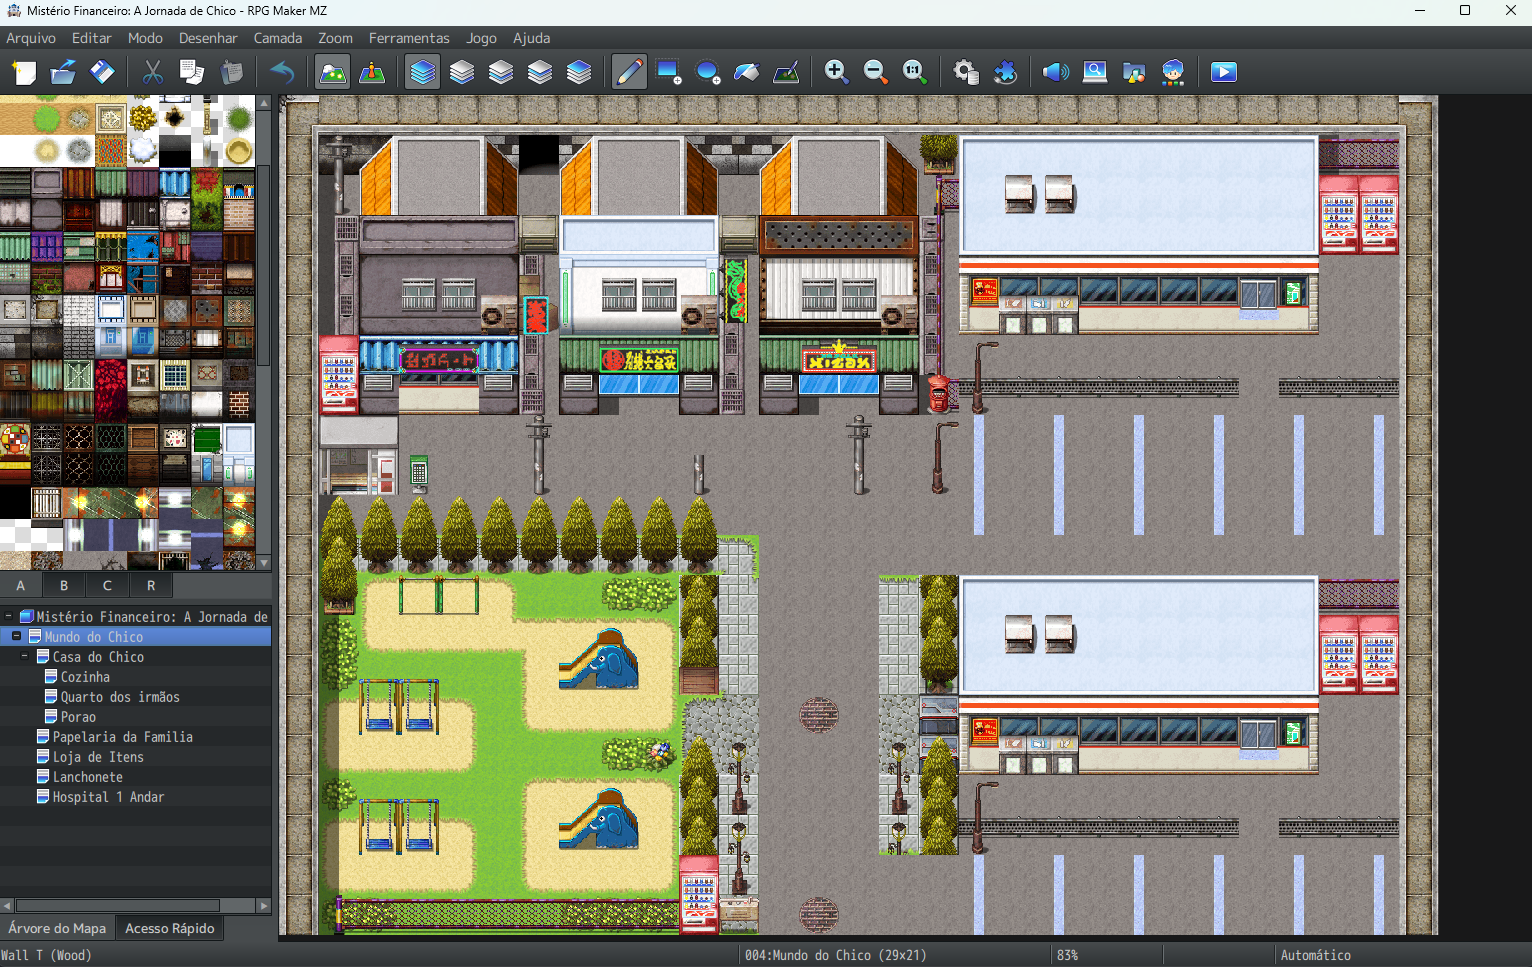
\includegraphics[scale=0.3]{Textuais/Pictures/RPGMaker_Interface.png}
	\fonte{Captura de tela do autor (2023).}\label{fig:rpgmaker-interface}
\end{figure}

%\subsection{Recursos e Funcionalidades}

O RPG Maker MZ oferece uma série de recursos que facilitam a criação de um ambiente educacional interativo. Entre eles, se destacam as funcionalidades detalhadas a seguir.

\icom{As figuras desta seção devem ser referenciadas e comentadas no texto (dizer o que elas apresentam, talvez dando exemplos de recursos interessantes/importantes para o seu trabalho).}

\subsubsection*{Comandos de evento}
Interface para criação de eventos que inclui exibição de texto, escolhas, controle de variáveis, e mais, facilitando a construção narrativa e interações no jogo.\com{Deixei só uma das três figuras. Uma alternativa é colocar as três imagens lado a lado, formando uma figura única com os comandos.} A Figura~\ref{fig:rpgmaker-event-commands-1} mostra...\com{Completar e fazer para or próximos...}

\begin{figure}[ht]
	\centering
	\caption{Alguns dos comandos de evento disponíveis no RPG Maker MZ.}
	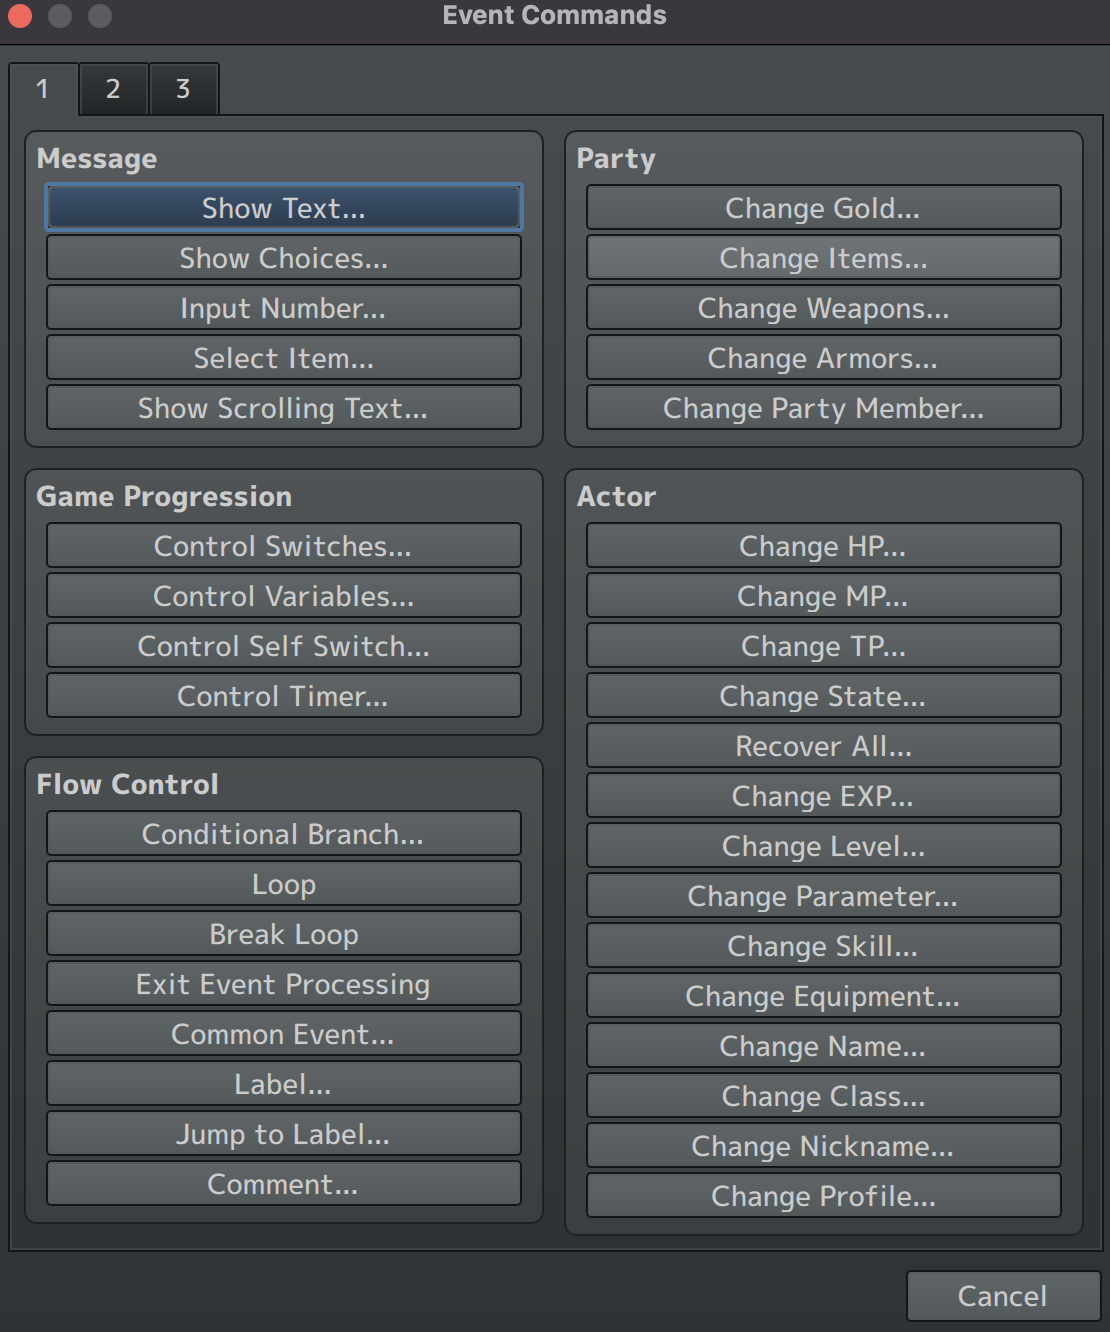
\includegraphics[scale=0.3]{Textuais/Pictures/Event-commands-1.png}
	\fonte{Captura de tela do autor (2023).}\label{fig:rpgmaker-event-commands-1}
\end{figure}

%\begin{figure}[ht]
%	\centering
%	\caption{Comandos disponíveis na página 2 do event commands do RPG Maker MZ.}
%	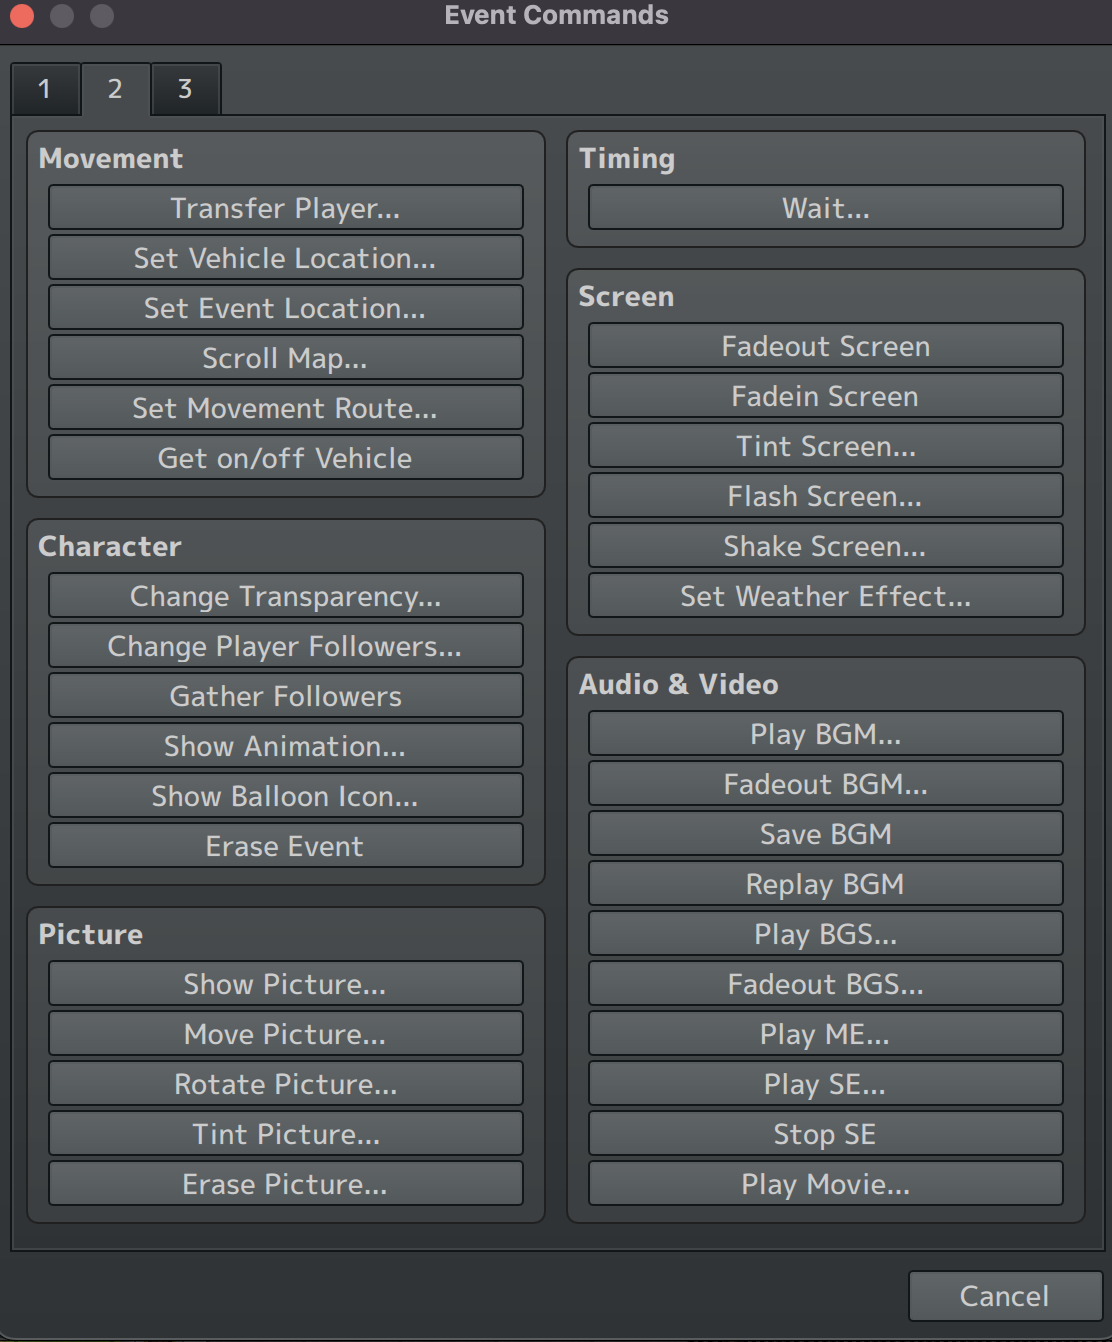
\includegraphics[scale=0.3]{Textuais/Pictures/Event-commands-2.png}
%	\fonte{Captura de tela do autor (2023).}\label{fig:rpgmaker-event-commands-2}
%\end{figure}
%
%\begin{figure}[ht]
%	\centering
%	\caption{Comandos disponíveis na página 3 do event commands do RPG Maker MZ.}
%	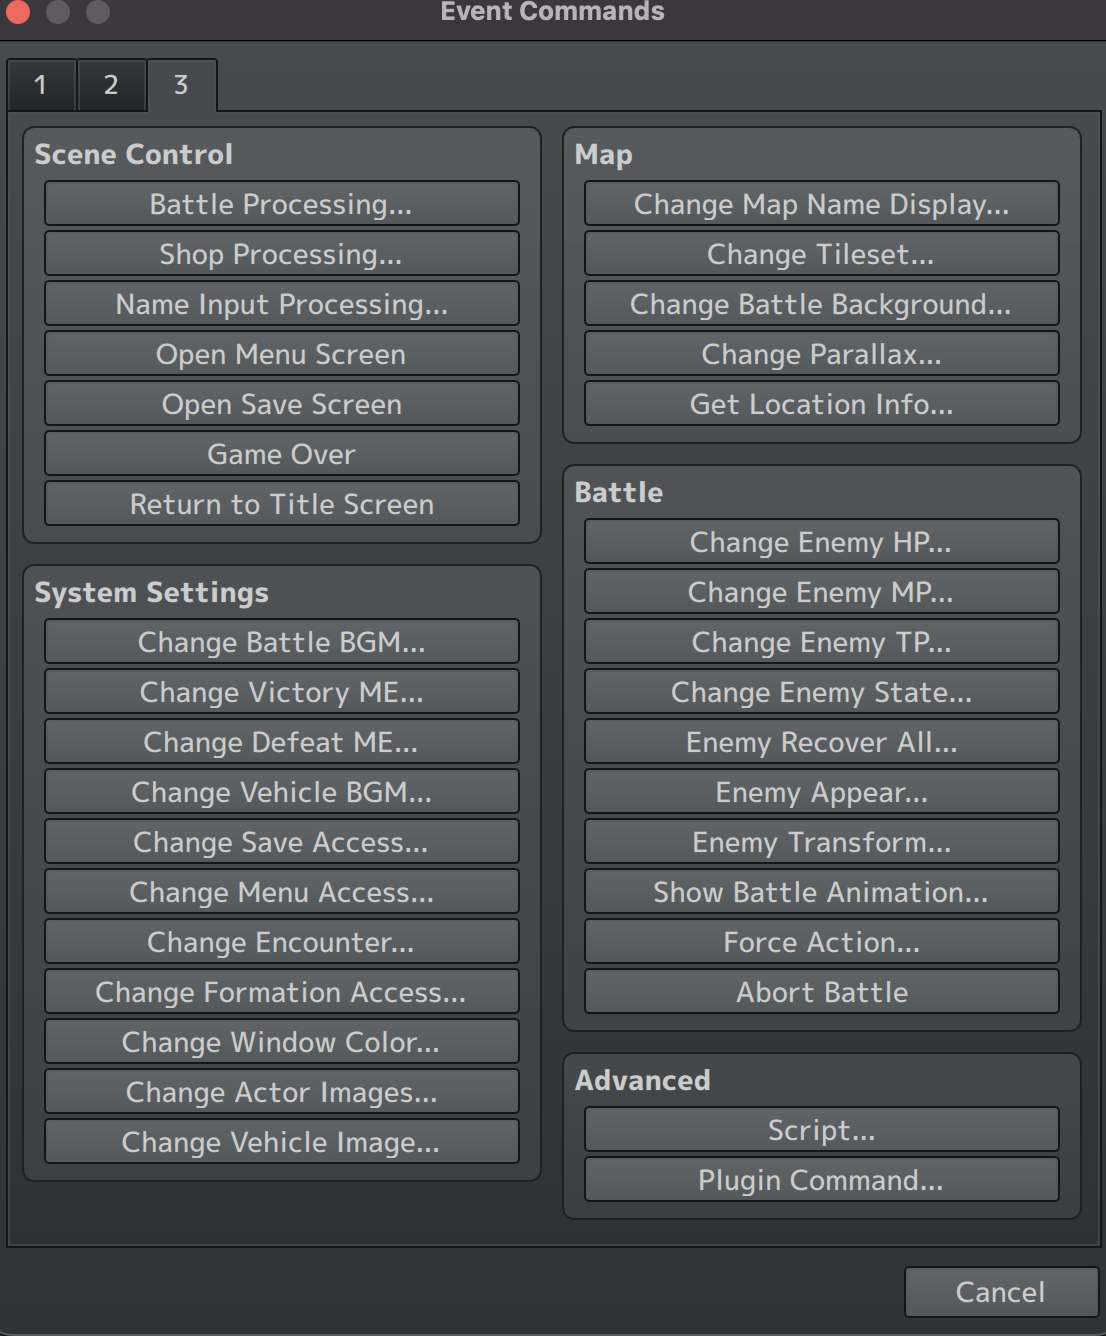
\includegraphics[scale=0.3]{Textuais/Pictures/Event-commands-3.png}
%	\fonte{Captura de tela do autor (2023).}\label{fig:rpgmaker-event-commands-3}
%\end{figure}

\subsubsection*{Criador de personagens}
Oferece um conjunto de ferramentas para a criação de personagens personalizados. Os usuários podem selecionar entre uma variedade de faces, cabelos, expressões, roupas e acessórios, permitindo uma personalização detalhada dos avatares do jogo.

\begin{figure}[ht]
	\centering
	\caption{Interface de criação de personagens do RPG Maker MZ.}
	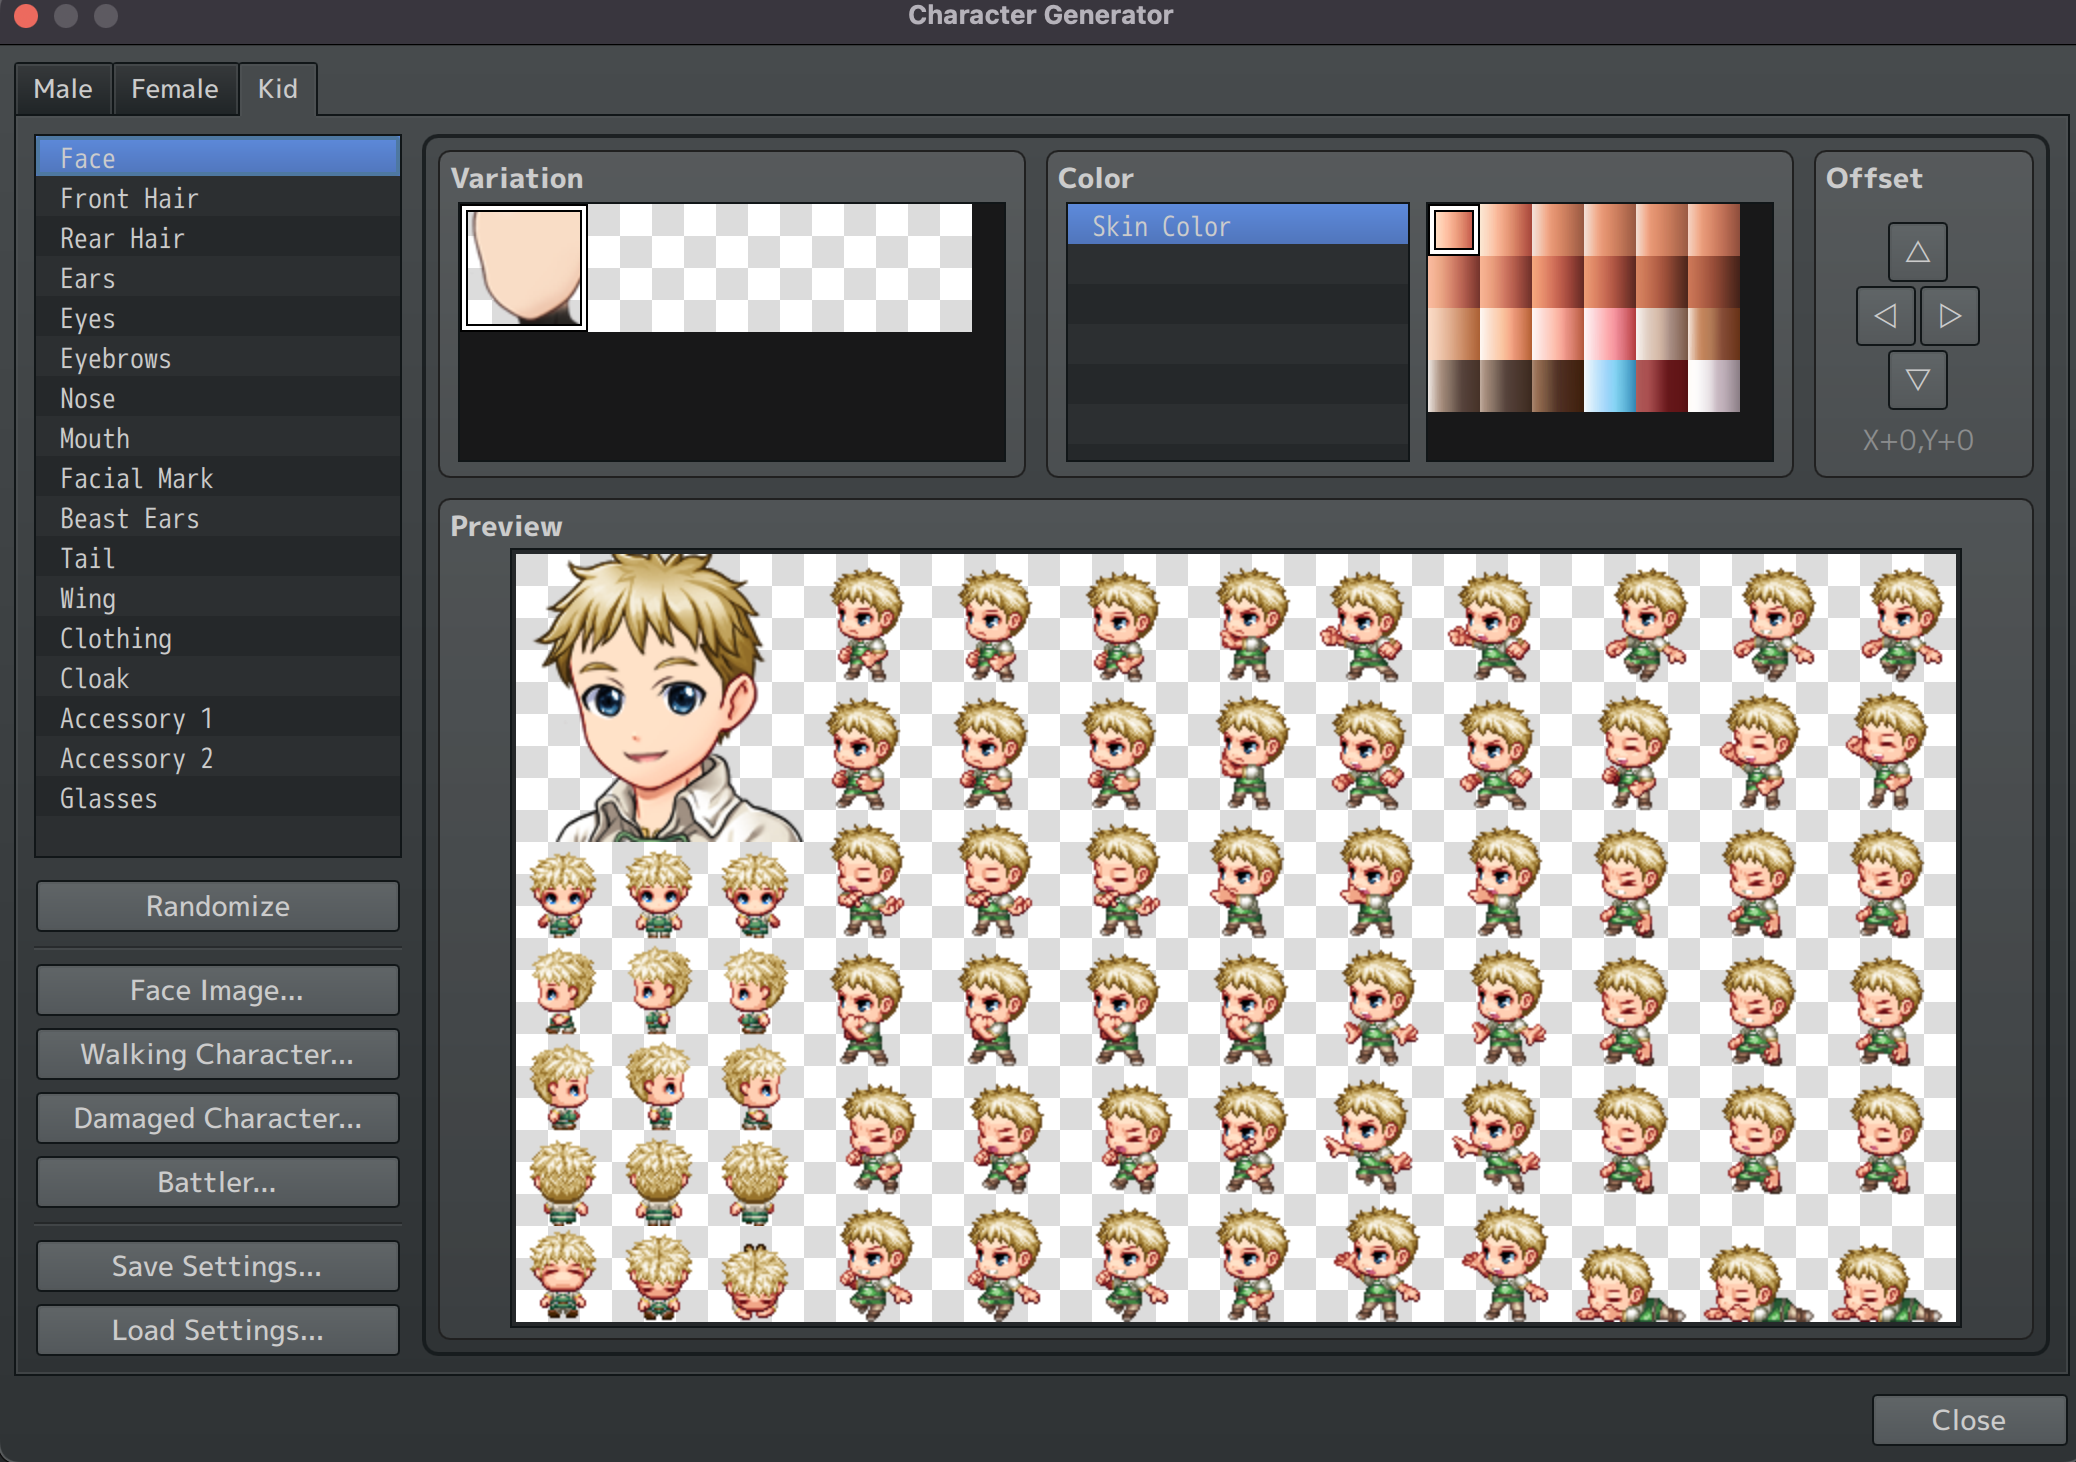
\includegraphics[scale=0.3]{Textuais/Pictures/Picture5.png}
	\fonte{Captura de tela do autor (2023).}\label{fig:rpgmaker-criador-personagens}
\end{figure}

\subsubsection*{Banco de dados}
Disponibiliza um banco de dados abrangente para o gerenciamento de elementos do jogo como itens, habilidades e inimigos, essencial para a criação de uma jogabilidade rica e envolvente.

\begin{figure}[ht]
	\centering
	\caption{Interface do Banco de dados do jogo no RPG Maker MZ.}
	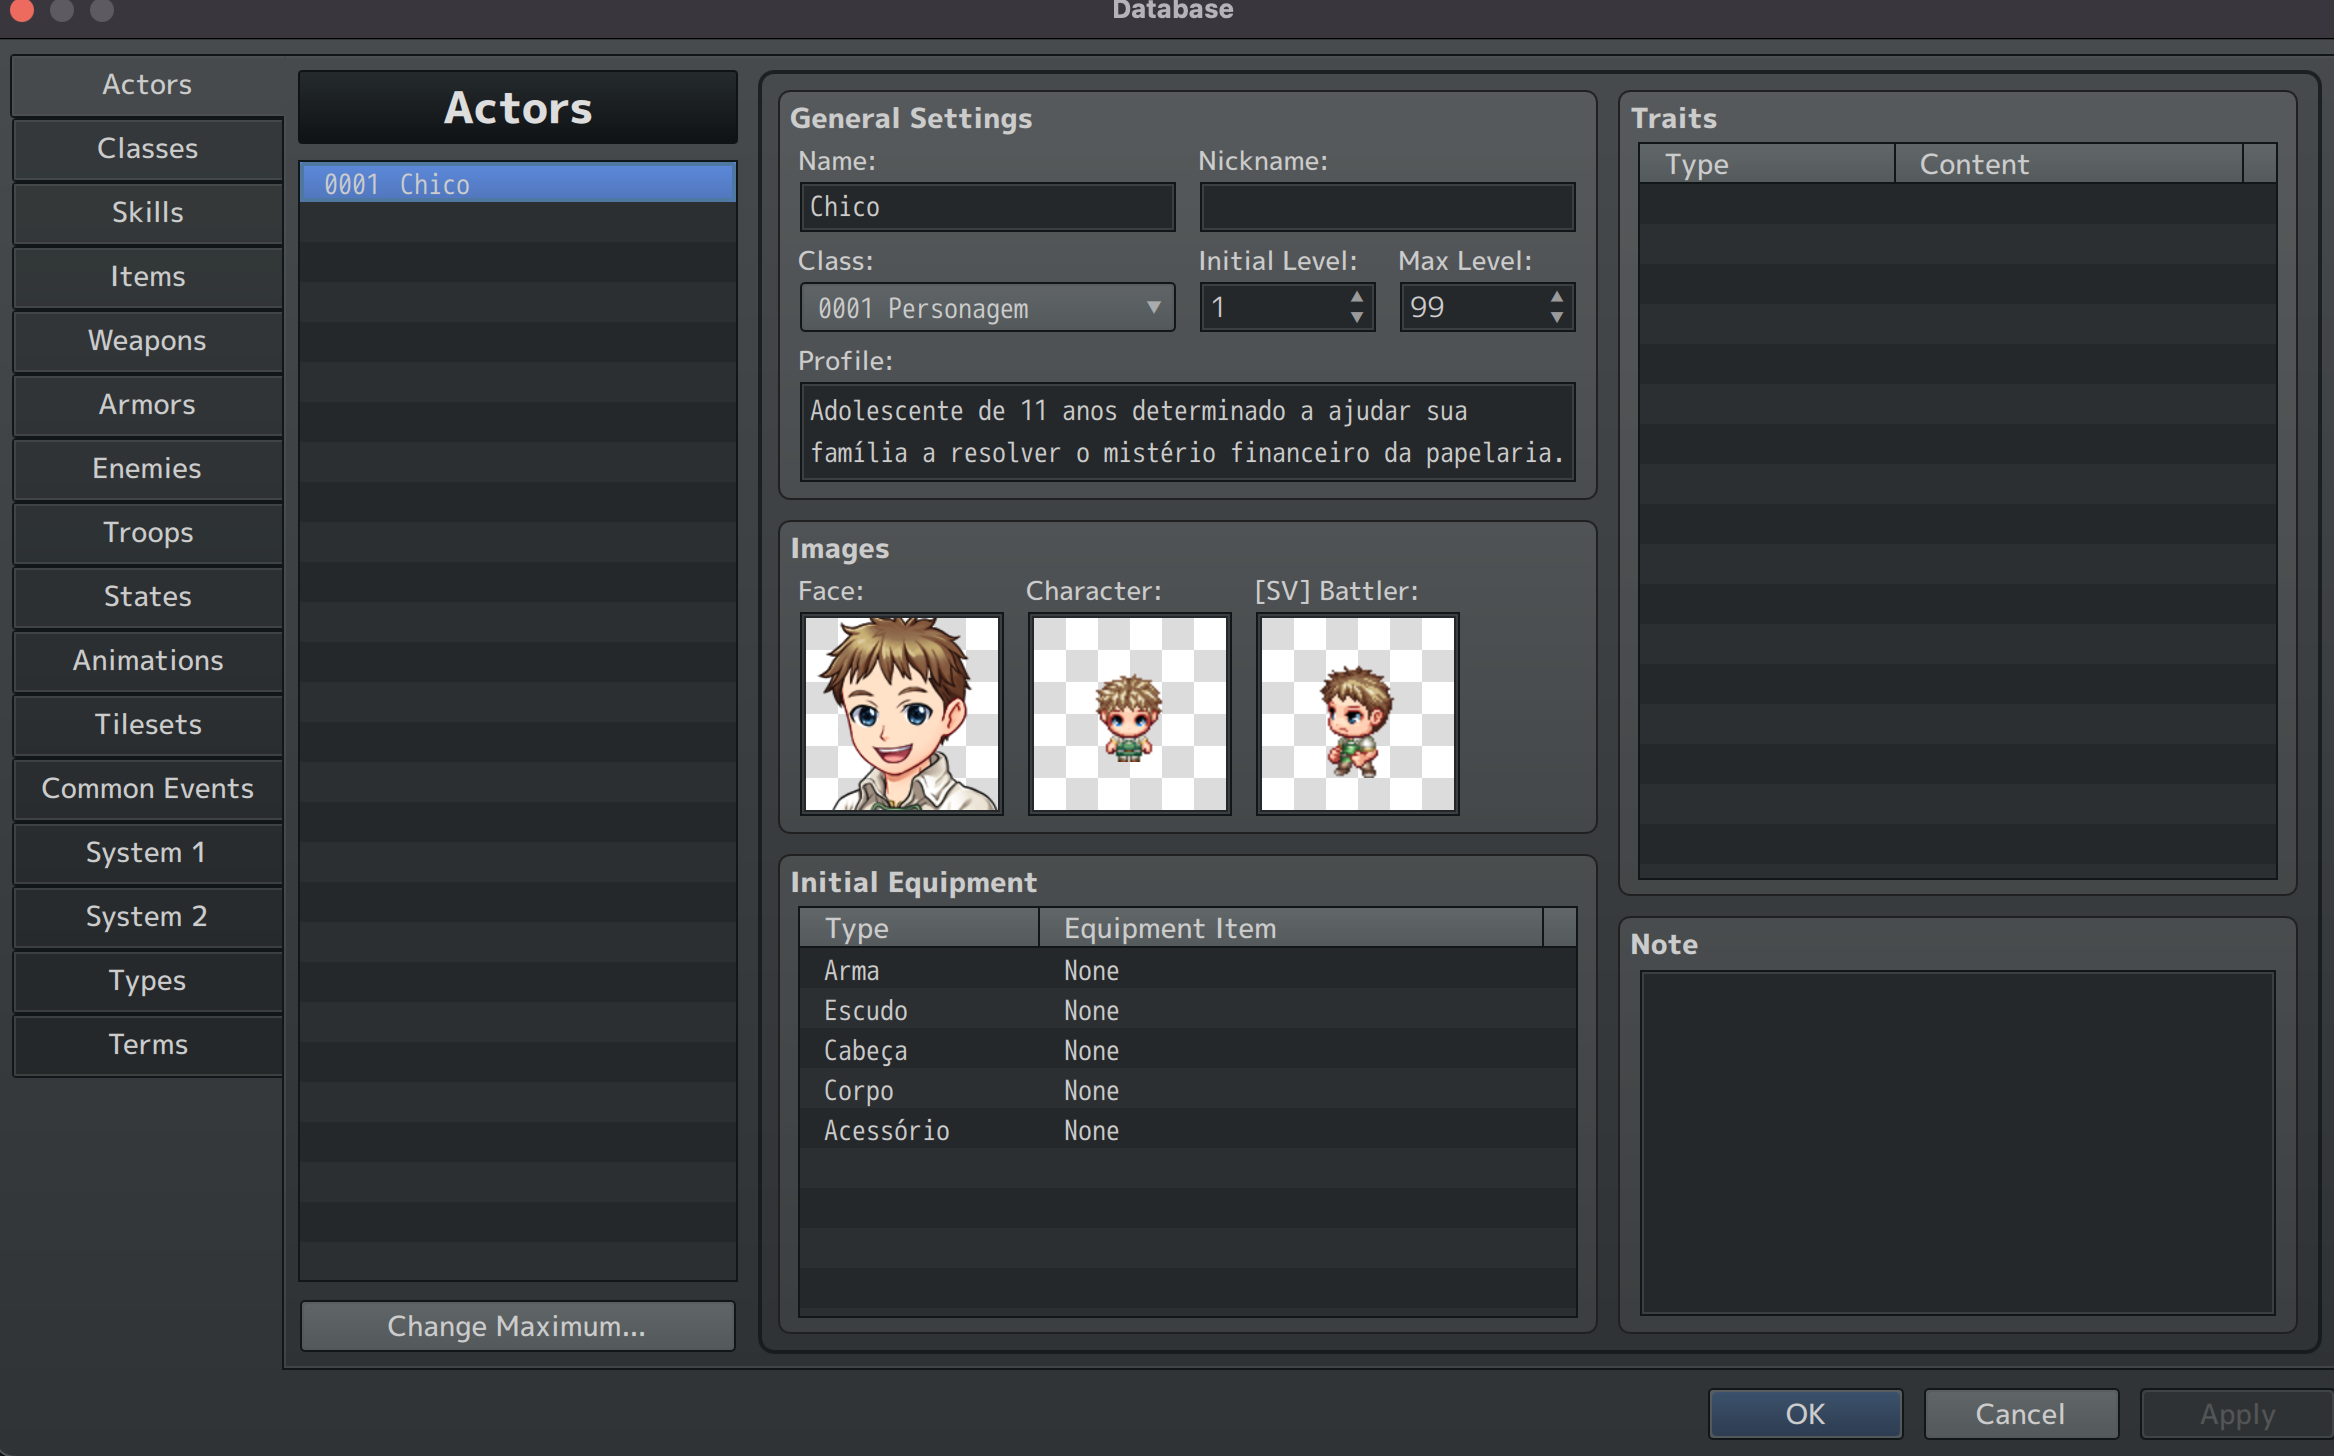
\includegraphics[scale=0.3]{Textuais/Pictures/DataBase.png}
	\fonte{Captura de tela do autor (2023).}\label{fig:rpgmaker-interface-database}
\end{figure}


\subsubsection*{Tilesets}
Disponibiliza uma vasta coleção de \textit{tilesets}, que são conjuntos de imagens usadas para construir os mapas do jogo, permitindo a criação de mundos detalhados e variados.

\begin{figure}[ht]
	\centering
	\caption{Interface de gestão de Tilesets do RPG Maker MZ.}
	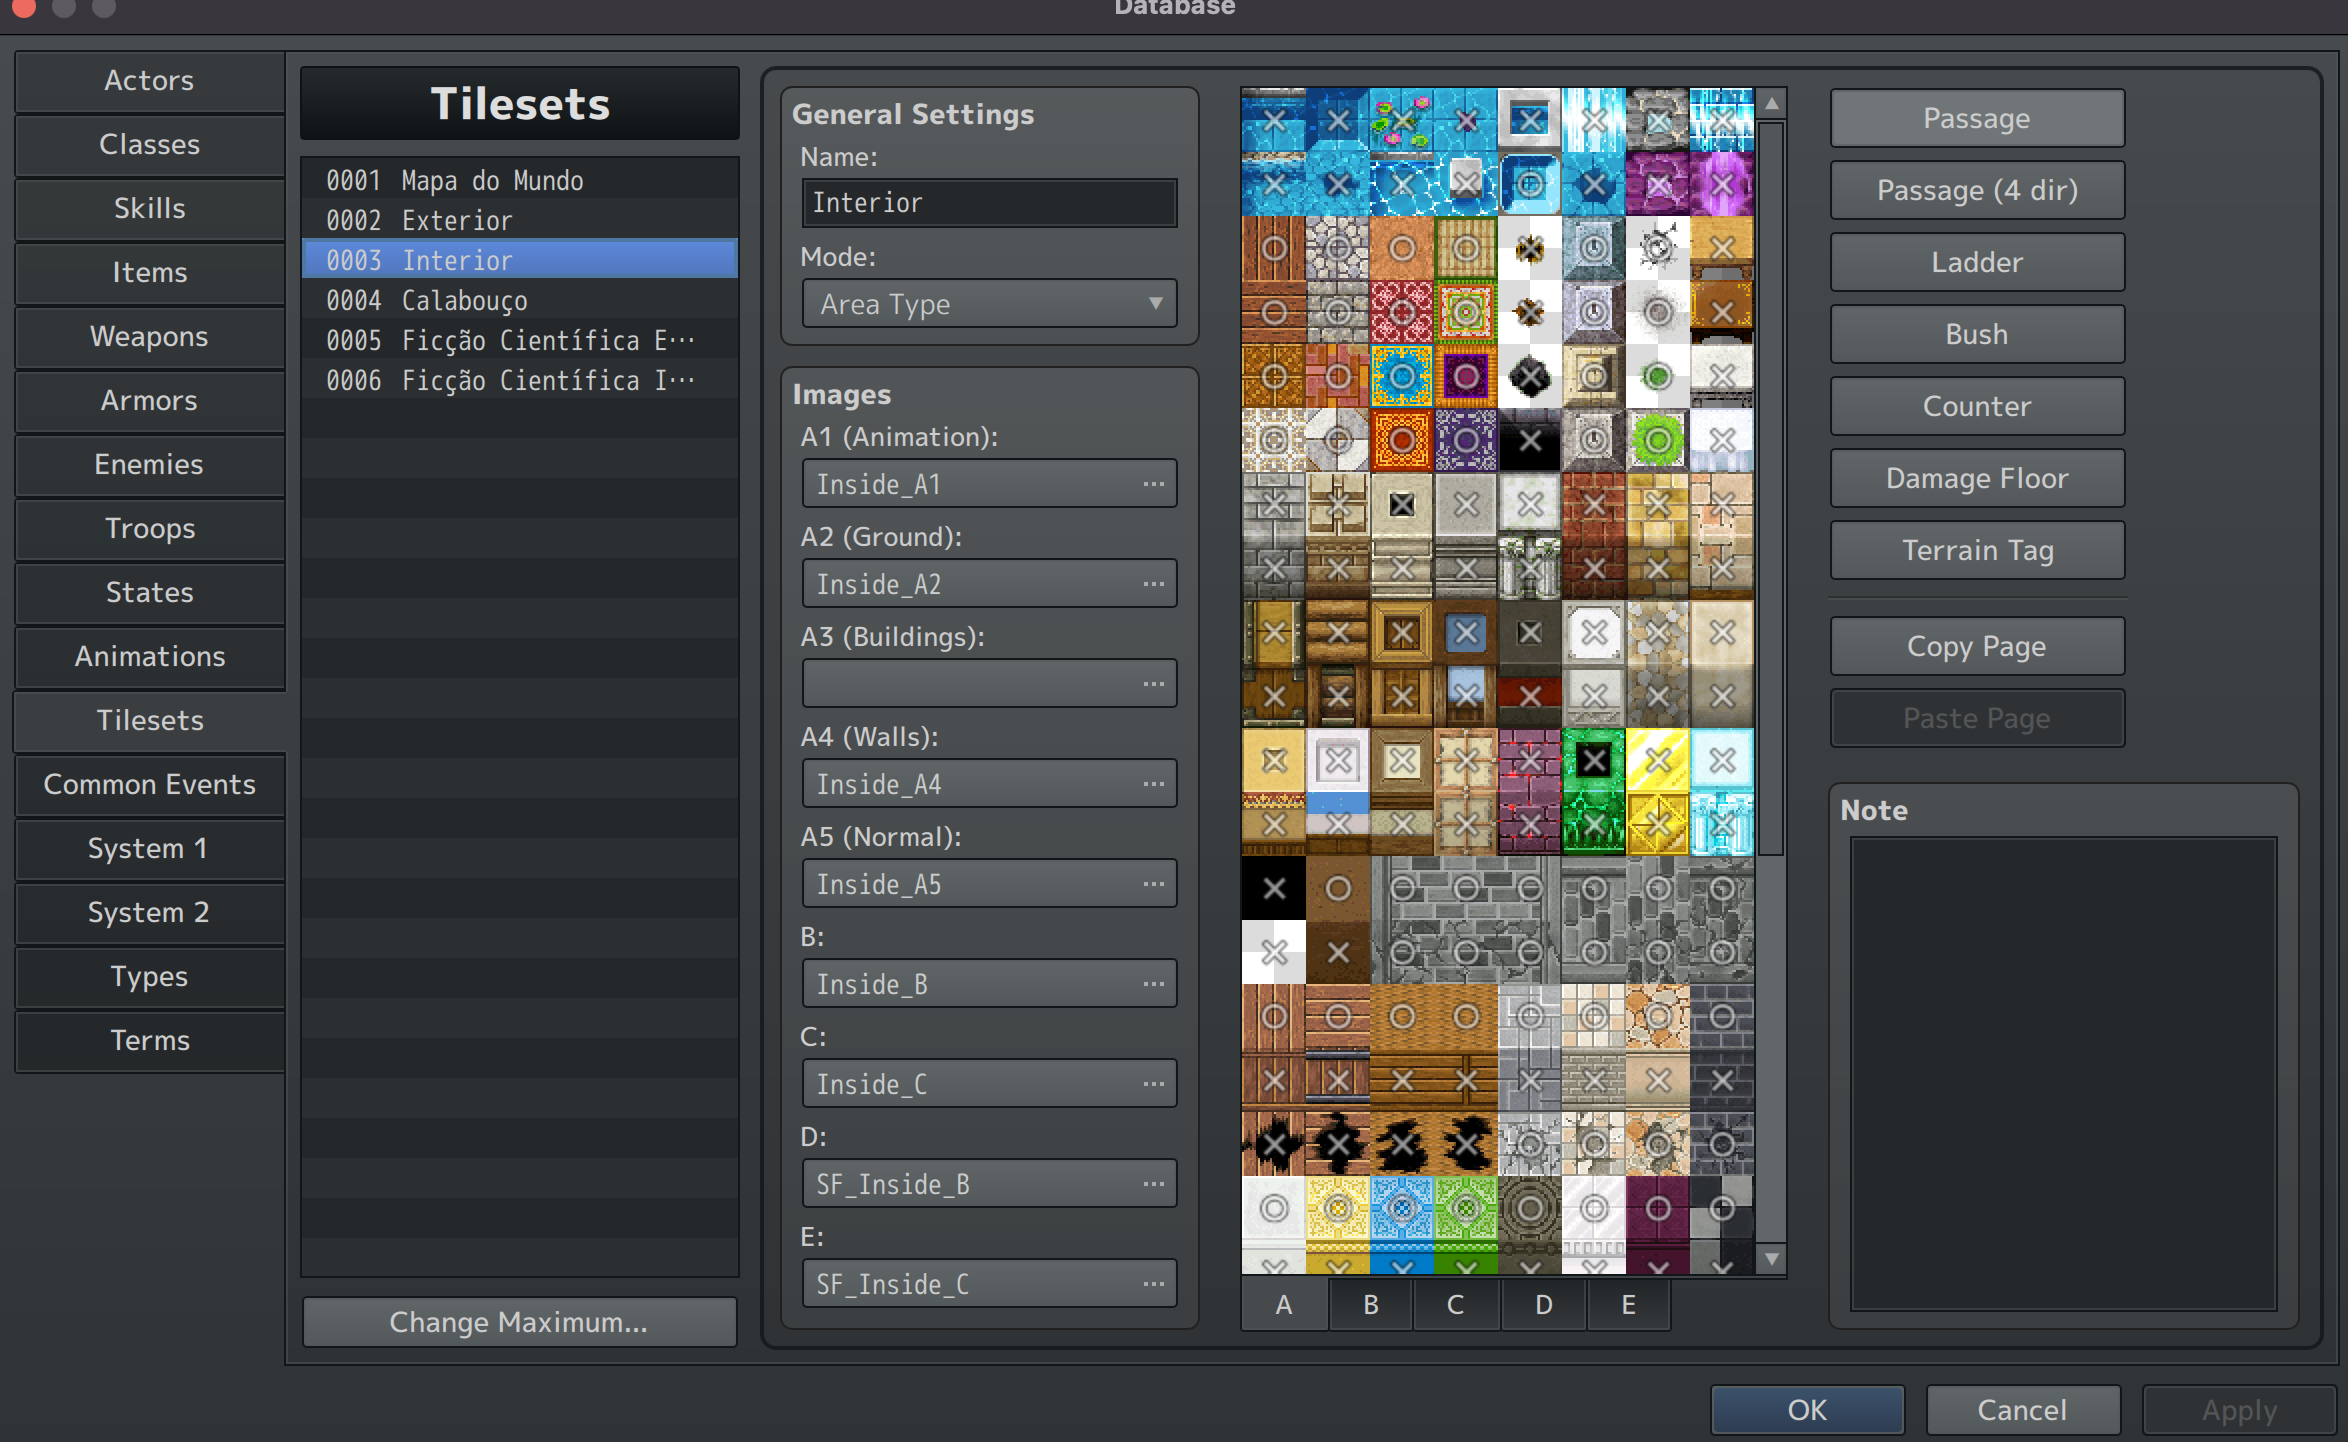
\includegraphics[scale=0.3]{Textuais/Pictures/Tileset.png}
	\fonte{Captura de tela do autor (2023).}\label{fig:rpgmaker-interface-tilesets}
\end{figure}


\section{GIMP}

O GIMP (\textit{GNU Image Manipulation Program}) é uma ferramenta de edição de imagens de código aberto, robusta e multiplataforma, que se revela uma escolha eficiente para a edição de \textit{tilesets} utilizados no RPG Maker MZ. Sua funcionalidade de manipulação de imagens permite aos desenvolvedores modificar e criar \textit{tilesets} personalizados, proporcionando um nível adicional de personalização e originalidade aos mapas do jogo. O GIMP suporta uma ampla gama de formatos de arquivo e oferece um leque de ferramentas de edição, desde simples cortes e ajustes de cores até operações complexas de manipulação de camadas e efeitos \cite{GIMP_Documentation}.

\begin{figure}[ht]
	\centering
	\caption{Interface de edição de imagem do GIMP.}
	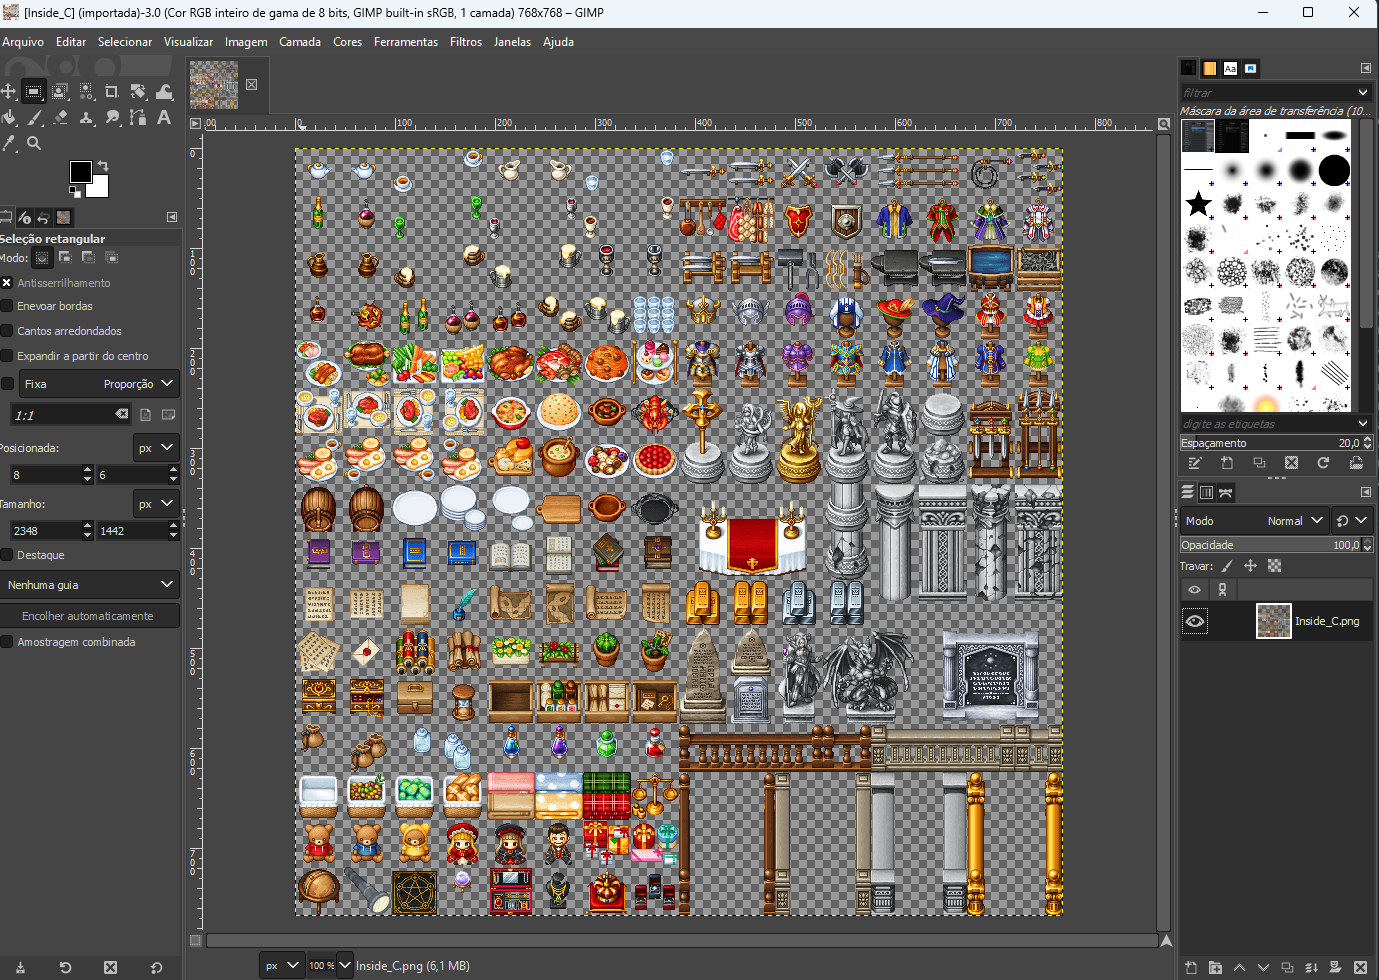
\includegraphics[scale=0.4]{Textuais/Pictures/Gimp.png}
	\fonte{Captura de tela do autor (2023).}\label{fig:gimp-interface}
\end{figure}

\icom{Depois de feitas as alterações sugeridas, o posicionamento de texto e figuras deverá ser ajustado.}


\section{Trabalhos Correlatos}
Esta seção apresenta alguns trabalhos que, de alguma forma, se correlacionam com o presente estudo, oferecendo uma perspectiva sobre as diversas abordagens em jogos educativos focados na educação financeira.

\subsection{Debt Maze}
O \textit{Debt Maze} \cite{Debt_Maze} representa um marco na integração de conceitos financeiros em jogos digitais. Esse jogo utiliza um labirinto repleto de desafios baseados em temas financeiros, como empréstimos, juros e pagamentos em atraso, criando uma experiência envolvente que se adapta a jogadores de diferentes níveis de conhecimento em finanças. A mecânica de navegação pelo labirinto simboliza as decisões financeiras na vida real, integrando elementos imersivos e persuasivos para educar e entreter o jogador. Essa abordagem lúdica contribui significativamente para a alfabetização financeira, incentivando decisões mais informadas.\com{É um jogo feito fora do Brasil? Se sim, pode comentar (no parágrafo abaixo) que seu jogo é focado no publico brasileiro, por seguir a ENEF e ser em português. Um jogo em inglês não é adequado para aplicação com estudantes brasileiros.}

Comparativamente, o presente trabalho distingue-se do \textit{Debt Maze} por adotar uma abordagem prática e cotidiana, mais adequada ao público infantil. Ao invés de um jogo de labirinto, propõe-se cenários reais e ferramentas interativas para simular decisões financeiras, aproximando o aprendizado à realidade das crianças. Além disso, por se basear na proposta da ENEF, o jogo desenvolvido neste trabalho é adequado para aplicação no ensino de educação financeira no Ensino Fundamental.

\icom{Mesmo comentário: as figuras precisam ser referenciadas e comentadas no texto (o que apresentam, etc).}

\icom{As duas figuras do Debt Maze têm o mesmo caption. Apresentar mais detalhes no caption, diferenciando as duas figuras, ou manter somente uma delas.}

\begin{figure}[ht]
	\centering
	\caption{Interface do Debt Maze.}
	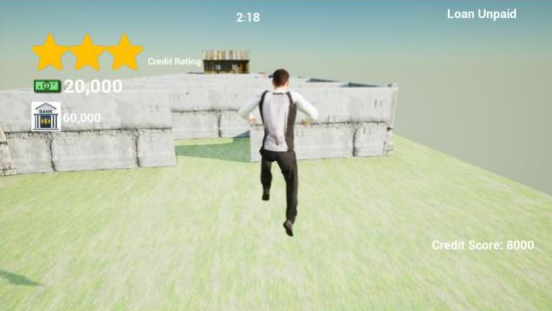
\includegraphics[scale=0.9]{Textuais/Pictures/debt-maze-1.png}
	\fonte{\textit{Debt Maze} \cite{Debt_Maze}.}\label{fig:debt-maze-1}
\end{figure}

\begin{figure}[ht]
	\centering
	\caption{Interface do Debt Maze.}
	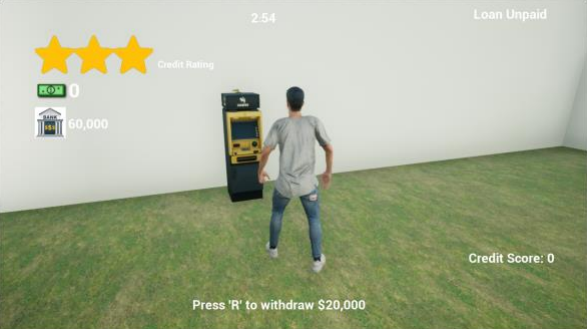
\includegraphics[scale=0.8]{Textuais/Pictures/debt-maze-2.png}
	\fonte{\textit{Debt Maze} \cite{Debt_Maze}.}\label{fig:debt-maze-2}
\end{figure}

\subsection{PlanCash}
O \textit{PlanCash} \cite{mariano2020educaccao}, um inovador jogo de tabuleiro, combina educação e entretenimento, utilizando a estrutura lúdica para ensinar matemática e gestão financeira a um público infantil. Este jogo aborda conceitos como a história do dinheiro e economia por meio de um tabuleiro interativo, onde os jogadores enfrentam situações-problema que estimulam a reflexão e análise financeiras. Essa abordagem didática destaca-se por integrar o aprendizado financeiro em atividades cotidianas, oferecendo uma base sólida para o entendimento infantil de conceitos financeiros e matemáticos.

Em contraste com esse jogo, o presente trabalho avança a ideia com uma proposta digital e atraente à geração atual de crianças, combinando elementos visuais e interativos para enriquecer a experiência educacional, alinhando o aprendizado financeiro às tecnologias contemporâneas.\com{Não está clara a diferença. Ambos são jogos digitais, certo? Então a diferença principal é o estilo RPG, que pode ser mais atrativo que um jogo digital no estilo de tabuleiro.}

\begin{figure}[ht]
	\centering
	\caption{Manual do \textit{PlanCash}.}
	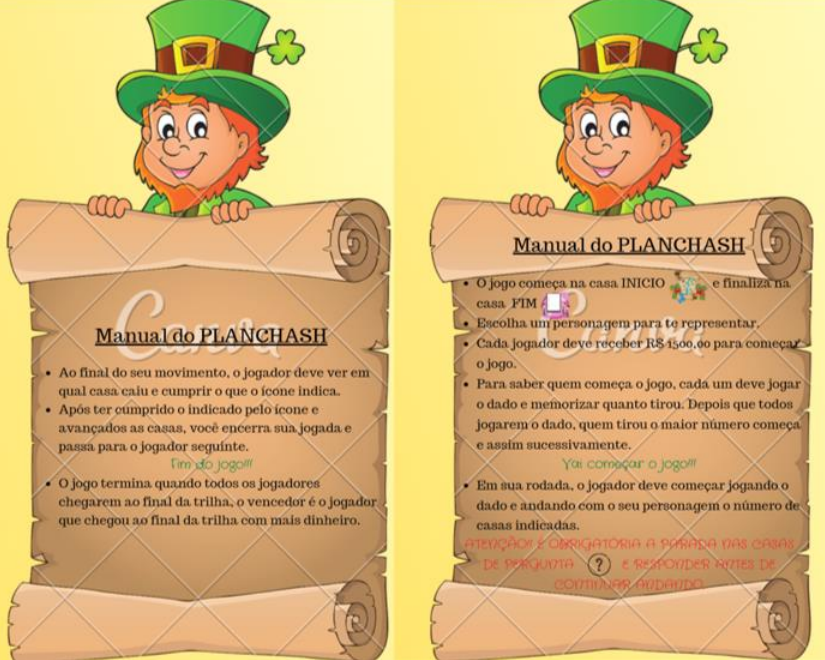
\includegraphics[scale=0.5]{Textuais/Pictures/Plancash-1.png}
	\fonte{\textit{PlanCash} \cite{mariano2020educaccao}.}\label{fig:plancash-1}
\end{figure}

\begin{figure}[ht]
	\centering
	\caption{Tabuleiro do \textit{PlanCash}.}
	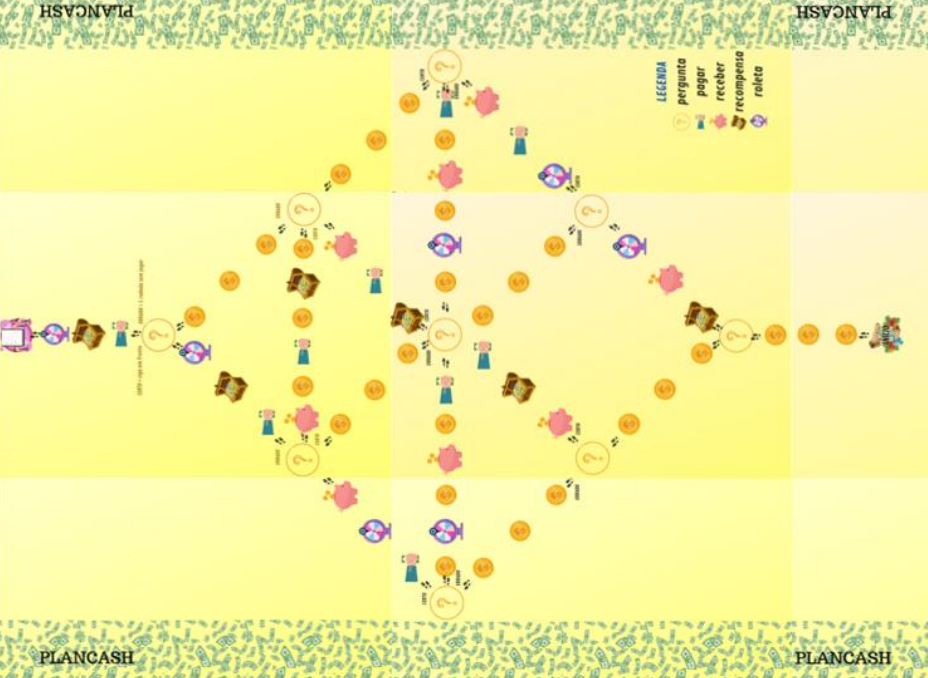
\includegraphics[scale=0.5]{Textuais/Pictures/Plancash-2.png}
	\fonte{\textit{PlanCash} \cite{mariano2020educaccao}.}\label{fig:plancash-2}
\end{figure}

\newpage

\subsection{Finance Game}

O \textit{Finance Game} \cite{Finance_Game} adota uma abordagem de simulação para a educação financeira, oferecendo aos jogadores cenários da vida adulta, como a gestão de um orçamento pessoal. Esse jogo destaca-se por seu foco na tomada de decisões financeiras equilibradas, promovendo um entendimento prático sobre responsabilidade financeira e bem-estar pessoal. A interação com elementos simulados do cotidiano, como mercado e banco, proporciona aos jogadores uma vivência educacional que transcende a mera teoria, enfatizando a importância de escolhas conscientes.

Em comparação, o presente trabalho foca em uma imersão mais alinhada à realidade infantil, oferecendo cenários e decisões financeiras que se conectam diretamente às experiências e compreensão das crianças, facilitando a assimilação dos conceitos de educação financeira.

\begin{figure}[ht]
	\centering
	\caption{Tela Inicial do \textit{Finance Game}.}
	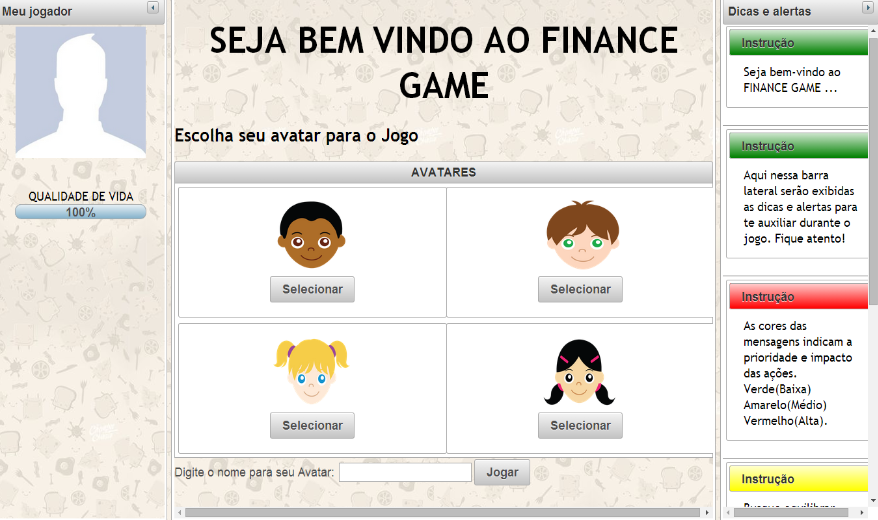
\includegraphics[scale=0.6]{Textuais/Pictures/Finance-game-1.png}
	\fonte{\textit{Finance Game} \cite{Finance_Game}.}\label{fig:finance-game-1}
\end{figure}

\begin{figure}[ht]
	\centering
	\caption{Cena do Mercado em \textit{Finance Game}.}
	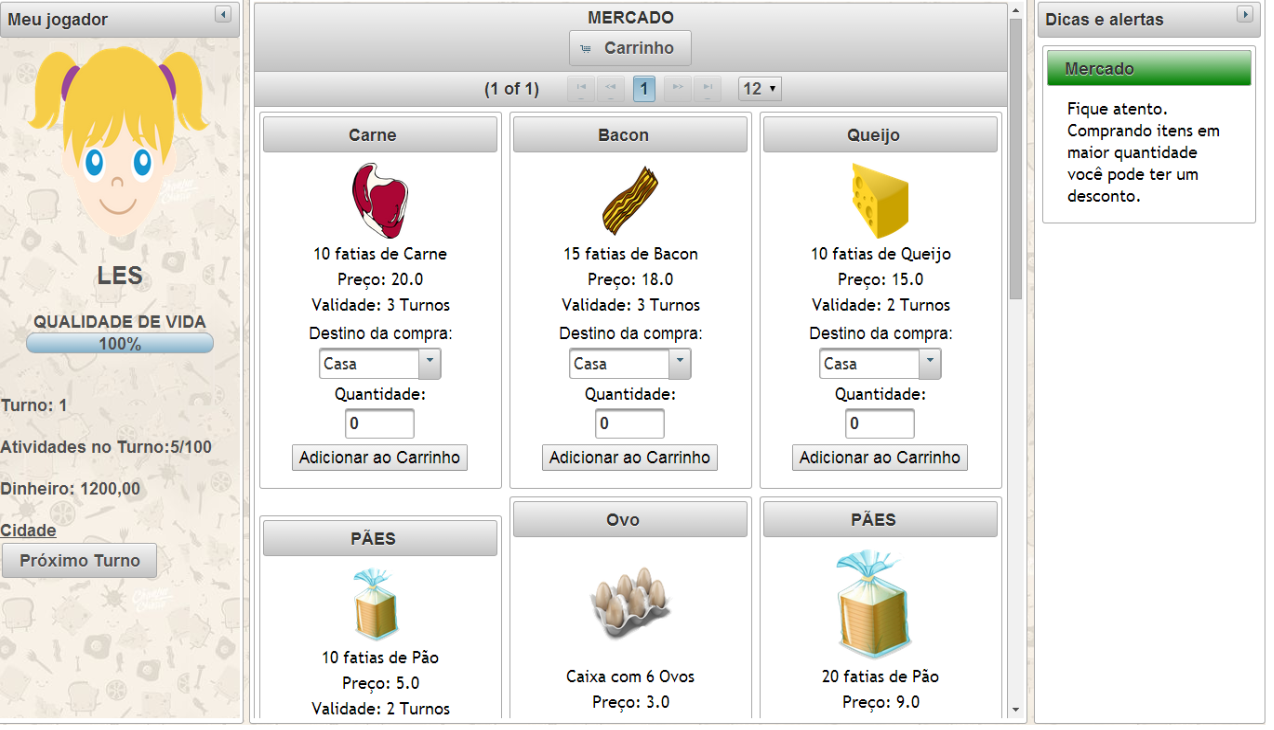
\includegraphics[scale=0.4]{Textuais/Pictures/Finance-game-2.png}
	\fonte{\textit{Finance Game} \cite{Finance_Game}.}\label{fig:finance-game-2}
\end{figure}

\newpage

\subsection{InvestPlay}
O \textit{InvestPlay} \cite{santos2020investplay} é um exemplo de jogo educativo que combina diversão e aprendizado em finanças. Esse jogo introduz os jogadores à gestão de ativos e passivos, adotando uma mecânica interativa de perguntas e respostas. O nível desafiador de algumas perguntas é uma consideração importante, especialmente para o público infantil. A personalização do jogo para diferentes temas educativos é um ponto forte, permitindo adaptar o conteúdo ao nível de compreensão das crianças.

Comparando-o com o presente estudo, busca-se refinar a proposta educacional do \textit{InvestPlay}, alinhando os conteúdos especificamente ao entendimento infantil. Esta abordagem simplificada visa tornar os conceitos financeiros mais acessíveis e relevantes para crianças, facilitando a assimilação eficaz dos princípios financeiros.\com{Além disso, um RPG é mais atrativo que um jogo de perguntas e respostas. Cabe pontuar essa diferença.}

\begin{figure}[ht]
	\centering
	\caption{Tela de instruções iniciais do \textit{InvestPlay}.}
	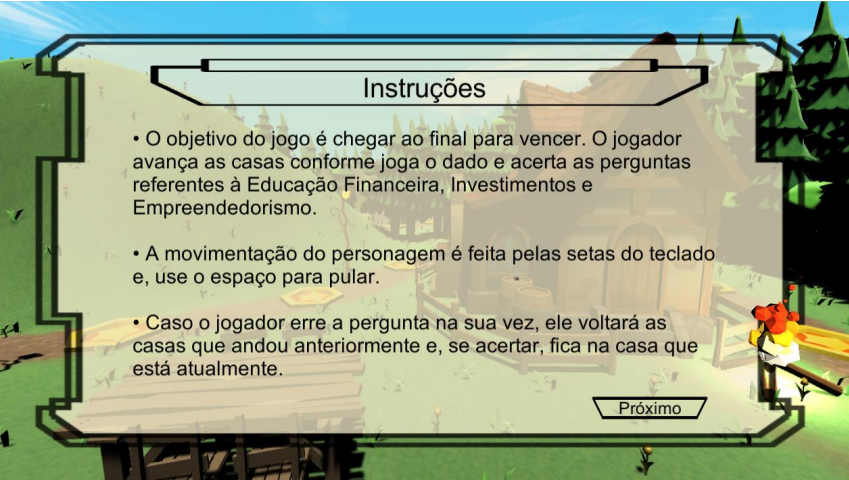
\includegraphics[scale=0.6]{Textuais/Pictures/invest-play-1.png}
	\fonte{\textit{InvestPlay} \cite{santos2020investplay}.}\label{fig:invest-play-1}
\end{figure}

\begin{figure}[ht]
	\centering
	\caption{Cena do jogo \textit{InvestPlay}.}
	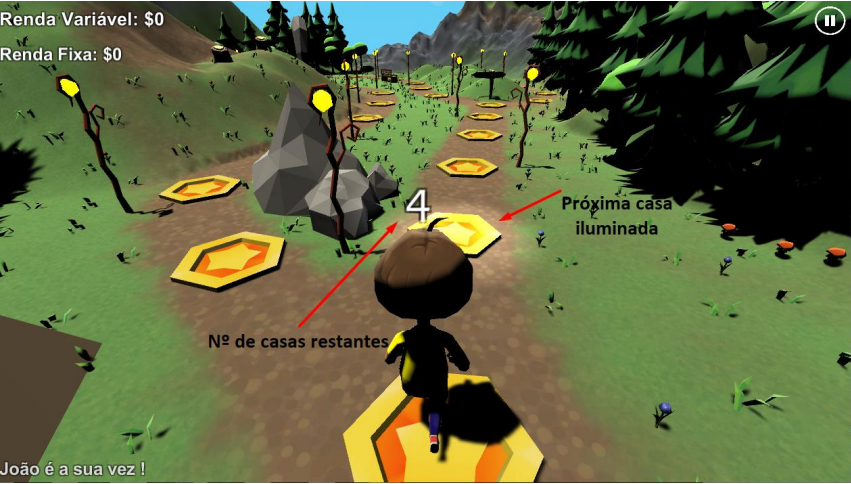
\includegraphics[scale=0.6]{Textuais/Pictures/invest-play-2.png}
	\fonte{\textit{InvestPlay} \cite{santos2020investplay}.}\label{fig:invest-play-2}
\end{figure}

\subsection{Considerações sobre os Trabalhos Correlatos}
Esta seção evidencia a diversidade de abordagens em jogos educativos focados em finanças, cada um com suas características distintas. A gamificação, como demonstrado nos exemplos citados, é uma ferramenta eficaz para a educação financeira, adaptando-se a diferentes públicos e objetivos de aprendizagem. No entanto, ressalta-se a importância de alinhar a metodologia e o conteúdo ao público-alvo, especialmente ao lidar com conceitos financeiros para crianças, onde a simplicidade e a relevância dos conteúdos são fundamentais.

\icom{Referenciar e comentar a tabela no texto.}

\begin{table}[ht]
	\centering
	\renewcommand{\arraystretch}{1.3}
	\caption{Comparativo Aprofundado dos Trabalhos Correlatos}
	\label{tab:comparativo-trabalhos}
	\begin{tabular}{| L{2.5cm} | L{2.6cm} | L{2.6cm} | L{2.6cm} | L{2.6cm} | L{2.6cm} |}
		\hline
		\textbf{}                       & \textbf{Debt Maze}       & \textbf{PlanCash}                    & \textbf{Finance Game}        & \textbf{InvestPlay}               \\
		\hline
		\hline
		\textbf{Público-Alvo}           & Geral                    & Infantil                             & Geral                        & Geral                             \\
		\hline
		\textbf{Metodologia}            & Labirinto                & Jogo de Tabuleiro                    & Simulação                    & Perguntas e Respostas             \\
		\hline
		\textbf{Abordagem Pedagógica}   & Gamificação              & Gamificação e Educação Tradicional   & Simulação Realista           & Dinâmica Interativa               \\
		\hline
		\textbf{Integração Tecnológica} & Média                    & Baixa                                & Média                        & Média                             \\
		\hline
		\textbf{Impacto Educacional}    & Alfabetização Financeira & Conhecimento Financeiro e Matemático & Tomada de Decisão Financeira & Entendimento de Ativos e Passivos \\
		\hline
		\textbf{Baseado na ENEF}        & Não                      & Não                                  & Não                          & Não                               \\
		\hline
	\end{tabular}
	\vspace{2mm}
	\fonte{Elaborado pelo autor (2023).}
\end{table}

\chapter{Desenvolvimento}

\section{Mistério Financeiro: A Jornada de Chico}

\subsection{Investigação Inicial}
No início do jogo, o protagonista Chico se depara com o mistério das despesas crescentes e do desaparecimento de moedas na papelaria de sua família. Motivado por um senso de responsabilidade, ele decide investigar, começando pelo porão da loja, um local pouco explorado.

\subsection{Desafios e Escolhas}
A narrativa avança através de uma série de desafios e escolhas que Chico deve enfrentar. Estas decisões vão desde escolhas cotidianas, como a compra de um relógio, até interações complexas com personagens como Vicente. Cada escolha tem um impacto significativo na história e nas lições de economia e gestão financeira apresentadas.

\subsection{Descobertas e Revelações}
À medida que Chico investiga, ele descobre várias causas para os problemas financeiros da papelaria, desde descuidos simples até ações mal-intencionadas de terceiros. O jogo ressalta a importância da atenção aos detalhes e do controle de gastos para a saúde financeira de um negócio.

\subsection{Interatividade e Impacto das Decisões}
"Mistério Financeiro: A Jornada de Chico" é estruturado de forma interativa, oferecendo múltiplos finais baseados nas decisões do jogador. Isso enfatiza a relevância de escolhas responsáveis e informadas, tanto no jogo quanto na vida real.

\subsection{Educação Financeira}
O jogo incorpora um forte elemento educacional, enfatizando conceitos de gestão financeira. Ensina sobre a importância do planejamento financeiro, economia e investimentos, incentivando os jogadores a refletir sobre suas próprias decisões financeiras.

\section{Requisitos do Jogo}

\subsection{Requisitos Funcionais}
\begin{itemize}
	\item RF1. O jogo deve oferecer uma interface gráfica interativa, simbolizando os diferentes ambientes da história de Chico.
	\item RF2. Incluir um sistema de diálogo interativo com NPCs, como Seu Mário, Vicente, Luiza, entre outros.
	\item RF3. Permitir que o jogador faça escolhas que influenciam o desenvolvimento da história e interações com NPCs.
	\item RF4. Permitir a compra e utilização de itens para progredir na narrativa, principalmente se tratando da Lanterna que será usada para verificar o porão.
	\item RF5. Apresentar múltiplos finais com base nas decisões tomadas pelo jogador, influenciadas pelas interações com NPCs.
	\item RF6. Incorporar elementos de educação financeira dentro da narrativa e desafios, utilizando situações da história de Chico como exemplos.
\end{itemize}

\subsection{Requisitos Não Funcionais}
\begin{itemize}
	\item RNF1. O jogo deve ter uma interface gráfica atrativa e intuitiva, adequada para a faixa etária do 5º ano.
	\item RNF2. O jogo deve ser otimizado para um desempenho fluido, sem atrasos ou erros técnicos.
	\item RNF3. O jogo deve ser compatível com a plataforma Windows.
	\item RNF4. O jogo deve ter uma trilha sonora e efeitos sonoros imersivos, complementando a experiência visual.
\end{itemize}

\subsection{Regras de Negócio}
\begin{itemize}
	\item RN1. A história deve se adaptar e mudar com base nas escolhas feitas pelo jogador. (RF3, RF5)
	\item RN2. Os desafios e enigmas devem ser integrados na história e contribuir para o aprendizado sobre finanças. (RF4, RF6)
	\item RN3. Os diálogos e interações com NPCs devem oferecer pistas e informações relevantes para a progressão da história. (RF2)
	\item RN4. O jogo deve promover a conscientização sobre gestão financeira e economia de forma lúdica e educativa. (RF6)
\end{itemize}

\subsection{NPCs e Mapas}
Esta seção detalha os personagens não jogáveis (NPCs) e os mapas que serão fundamentais para a narrativa e jogabilidade do jogo. Cada NPC e mapa pode ser acompanhado de uma imagem e uma descrição detalhada para melhor imersão e compreensão do jogador.

\subsubsection{NPCs}
\begin{itemize}
	\item Seu Mário: Pai de Chico, dedicado dono da papelaria da família. Enfrenta desafios financeiros e tenta manter o negócio próspero.
	      \begin{figure}[ht]
		      \centering
		      \caption{NPC Seu Mário.}
		      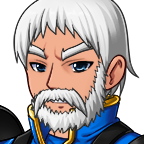
\includegraphics[scale=0.8]{Textuais/Pictures/Seu_Mario.png}
		      \fonte{Criado pelo Autor.}\label{fig:npc-seu-mario}
	      \end{figure}
	\item Pai do Vicente: Aparece na história para repreender seu filho por envolvimento em furtos, refletindo preocupação paterna.
	      \begin{figure}[ht]
		      \centering
		      \caption{NPC Pai do Vicente.}
		      
\includegraphics[scale=0.8]{Textuais/Pictures/Pai_Vicente.png}
		      \fonte{Criado pelo Autor.}\label{fig:npc-pai-vicente}
	      \end{figure}
	\item Atendente da Loja de Itens: Caracterizado como um comerciante prestativo, interage com Chico durante a compra do seu relógio.
	      \begin{figure}[ht]
		      \centering
		      \caption{NPC Atendente da Loja de Itens.}
		      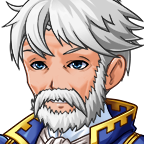
\includegraphics[scale=0.8]{Textuais/Pictures/Atendente_loja_Itens.png}
		      \fonte{Criado pelo Autor.}\label{fig:npc-atendente-loja-itens}
	      \end{figure}

	      \newpage

	\item Vicente: Colega de escola de Chico, conhecido por seu comportamento provocativo e envolvimento em pequenos furtos.
	      \begin{figure}[ht]
		      \centering
		      \caption{NPC Vicente.}
		      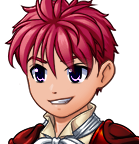
\includegraphics[scale=0.8]{Textuais/Pictures/Vicente.png}
		      \fonte{Criado pelo Autor.}\label{fig:npc-vicente}
	      \end{figure}
	\item Luiza: Melhor amiga de Chico, sempre oferecendo apoio e aconselhamento nas aventuras e desafios enfrentados por ele.
	      \begin{figure}[ht]
		      \centering
		      \caption{NPC Luiza.}
		      \includegraphics[scale=0.8]{Textuais/Pictures/Luísa.png}
		      \fonte{Criado pelo Autor.}\label{fig:npc-luiza}
	      \end{figure}
	\item Unnamed 1, 2, 3, 4: Personagens secundários, aparecem apenas para ilustrar algumas cenas como o encontro com o pessoal da escola na lanchonete.
	\item Maria José: Mãe de Chico, auxilia na papelaria e compartilha das preocupações financeiras da família.
	      \begin{figure}[ht]
		      \centering
		      \caption{NPC Maria José.}
		      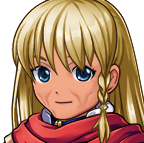
\includegraphics[scale=0.8]{Textuais/Pictures/Maria.png}
		      \fonte{Criado pelo Autor.}\label{fig:npc-maria-jose}
	      \end{figure}

	      \newpage

	\item Josimar: Funcionário da papelaria, inicialmente suspeito de furto, revelando-se inocente e um aliado importante.
	      \begin{figure}[ht]
		      \centering
		      \caption{NPC Josimar.}
		      
\includegraphics[scale=0.8]{Textuais/Pictures/Josimar.png}
		      \fonte{Criado pelo Autor.}\label{fig:npc-josimar}
	      \end{figure}
	\item Ratazana: Uma ameaça inesperada no porão da papelaria, adicionando suspense e desafios físicos à narrativa.
	      \begin{figure}[ht]
		      \centering
		      \caption{NPC Ratazana.}
		      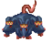
\includegraphics[scale=1.8]{Textuais/Pictures/Ratazana.png}
		      \fonte{Hellpug/Emily Lampson.}\label{fig:npc-ratazana}
	      \end{figure}
	\item Atendente do Hospital: Representa um ponto de contato no cenário hospitalar, caso Chico necessite de cuidados médicos.
	      \begin{figure}[ht]
		      \centering
		      \caption{NPC Atendente do Hospital.}
		      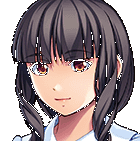
\includegraphics[scale=0.8]{Textuais/Pictures/Atendente_Hospital.png}
		      \fonte{\textit{Asset} padrão do RPG Maker MZ.}\label{fig:npc-atendente-hospital}
	      \end{figure}

	      \newpage

	\item Médico: Figura de cuidado e autoridade, que atende Chico no hospital após eventuais incidentes.
	      \begin{figure}[ht]
		      \centering
		      \caption{NPC Médico.}
		      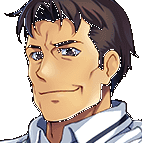
\includegraphics[scale=0.8]{Textuais/Pictures/Medico.png}
		      \fonte{\textit{Asset} padrão do RPG Maker MZ.}\label{fig:npc-medico}
	      \end{figure}
	\item Atendente da Loja de Ferragens: Ajuda Chico na aquisição da lanterna necessária para suas investigações.
	      \begin{figure}[ht]
		      \centering
		      \caption{NPC Atendente da Loja de Ferragens.}
		      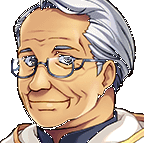
\includegraphics[scale=0.8]{Textuais/Pictures/Atendente_Loja_Ferragens.png}
		      \fonte{\textit{Asset} padrão do RPG Maker MZ.}\label{fig:npc-atendente-loja-ferragens}
	      \end{figure}
	\item Cida: Irmã mais nova de Chico, envolvida nos dilemas familiares e curiosa sobre os mistérios da papelaria.
	      \begin{figure}[ht]
		      \centering
		      \caption{NPC Cida.}
		      
\includegraphics[scale=0.8]{Textuais/Pictures/Cida.png}
		      \fonte{Criado pelo autor.}\label{fig:npc-cida}
	      \end{figure}
\end{itemize}

\newpage

\subsubsection{Mapas}
\begin{itemize}
	\item Mundo do Chico: O cenário geral da aventura, incluindo a vizinhança, ruas, e locais frequentados por Chico e seus amigos.

	      \begin{figure}[ht]
		      \centering
		      \caption{Mapa Mundo Chico.}
		      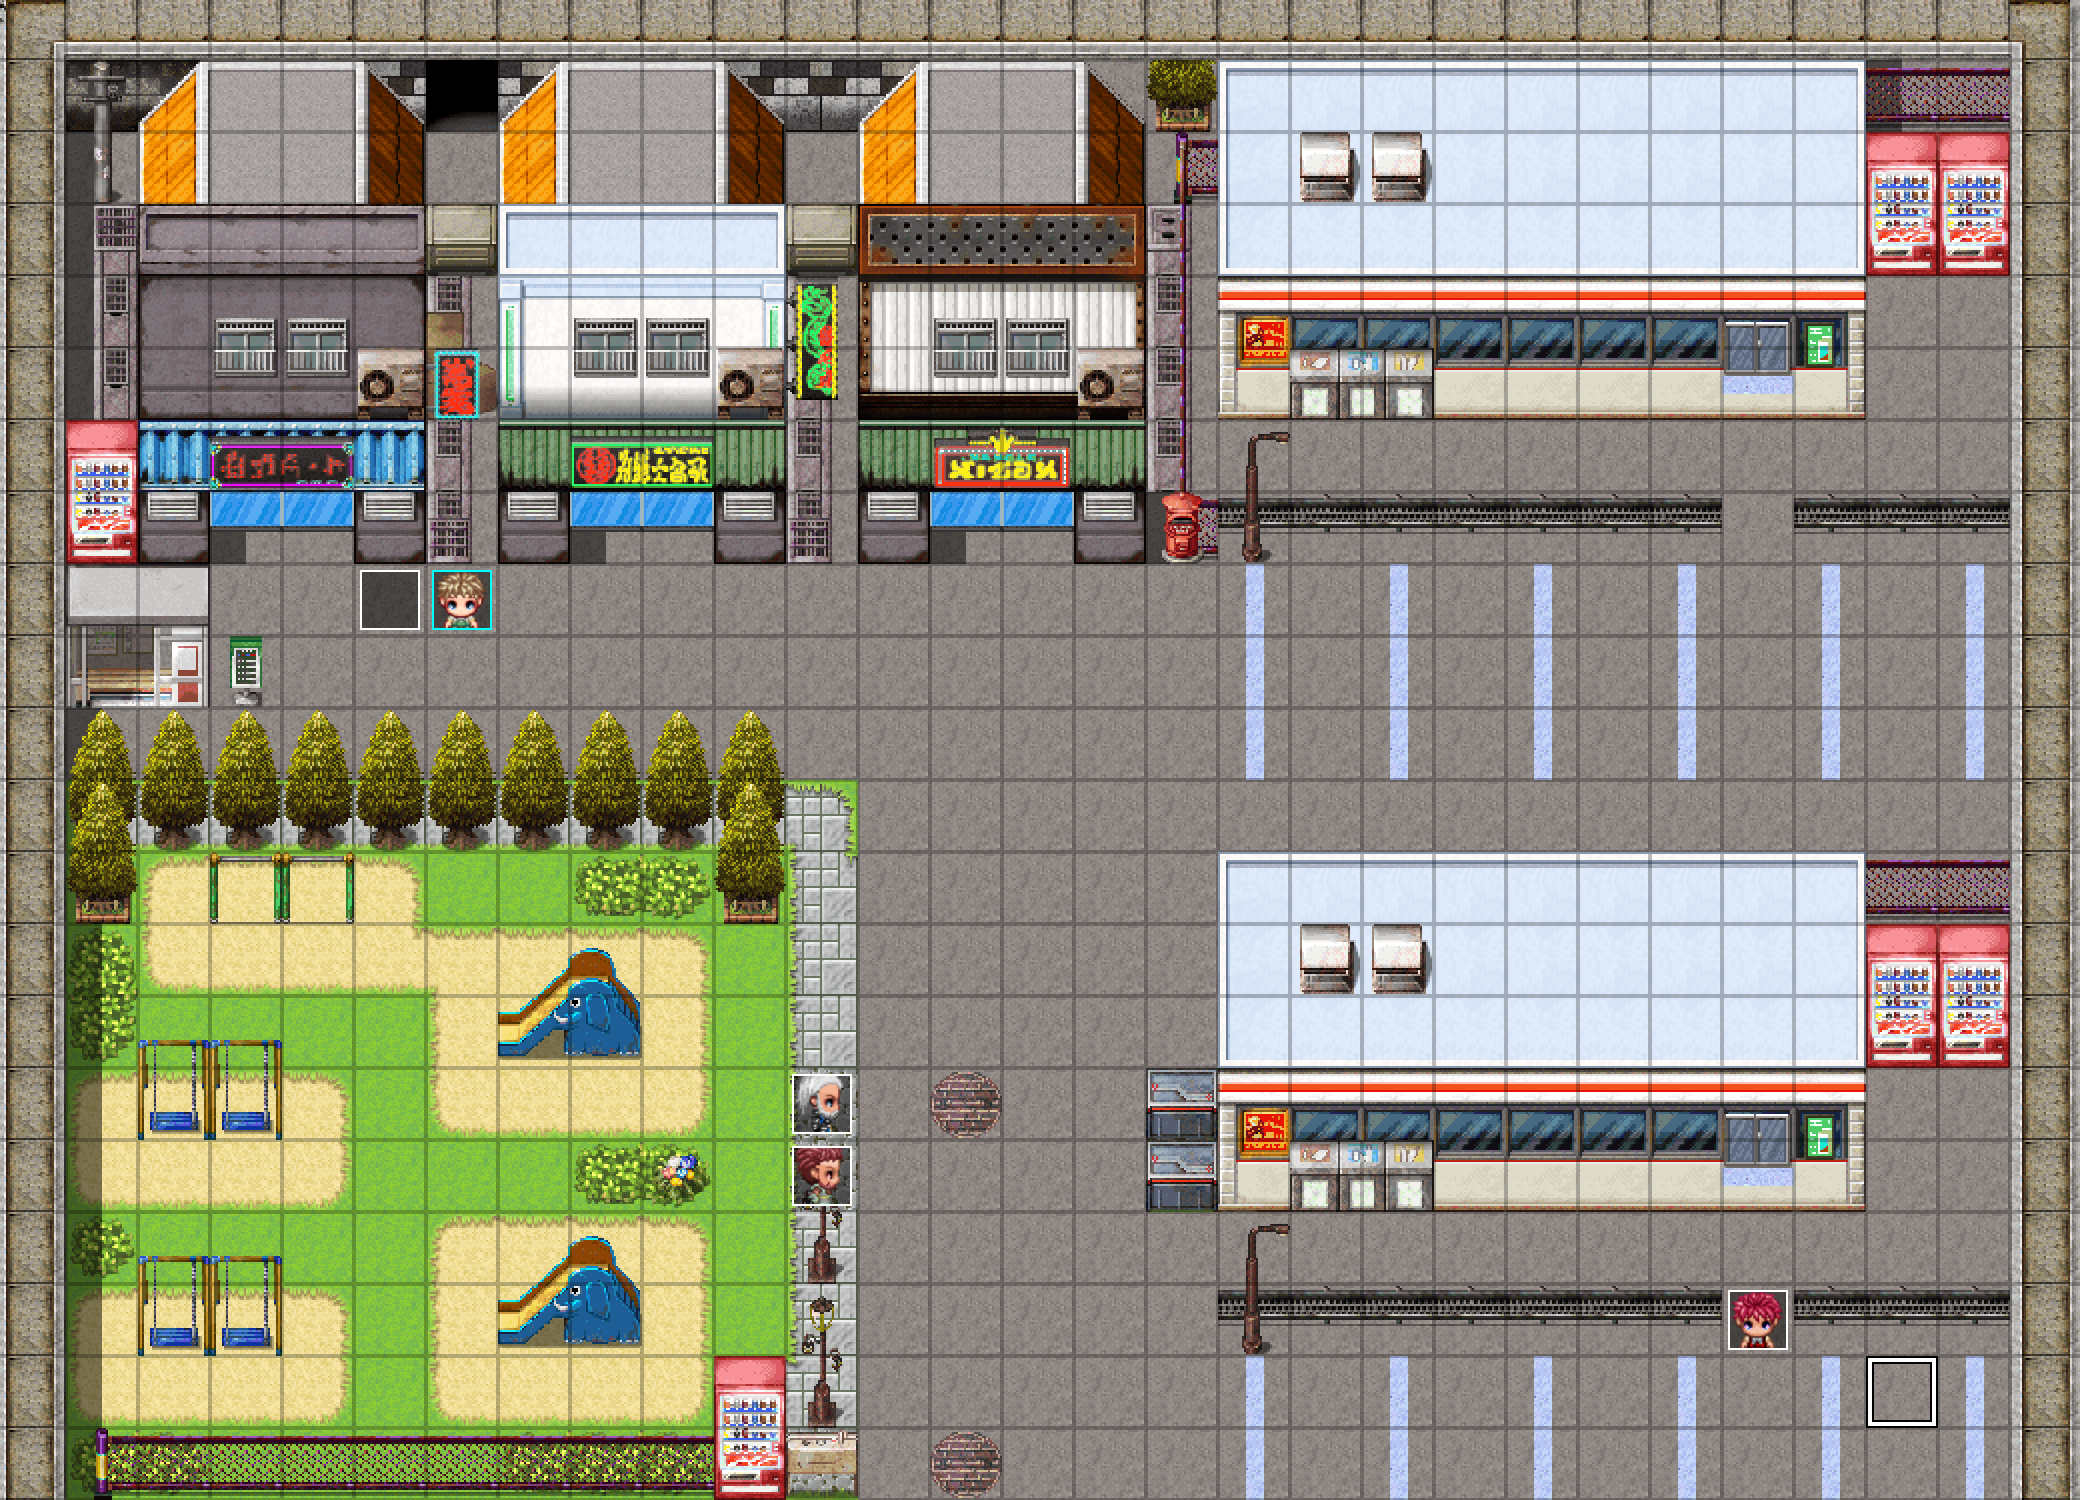
\includegraphics[scale=0.3]{Textuais/Pictures/Mundo_chico.png}
		      \fonte{Criado pelo autor.}\label{fig:mundo-chico}
	      \end{figure}


	\item Loja de Itens: Estabelecimento onde Chico adquire itens como o relógio.

	      \begin{figure}[ht]
		      \centering
		      \caption{Mapa Loja de Itens.}
		      \includegraphics[scale=0.4]{Textuais/Pictures/Loja_itens.png}
		      \fonte{Criado pelo autor.}\label{fig:loja-itens}
	      \end{figure}

	      \newpage

	\item Lanchonete: Espaço social para Chico e seus amigos, propício para conversas e desenvolvimento de subtramas.

	      \begin{figure}[ht]
		      \centering
		      \caption{Mapa Lanchonete.}
		      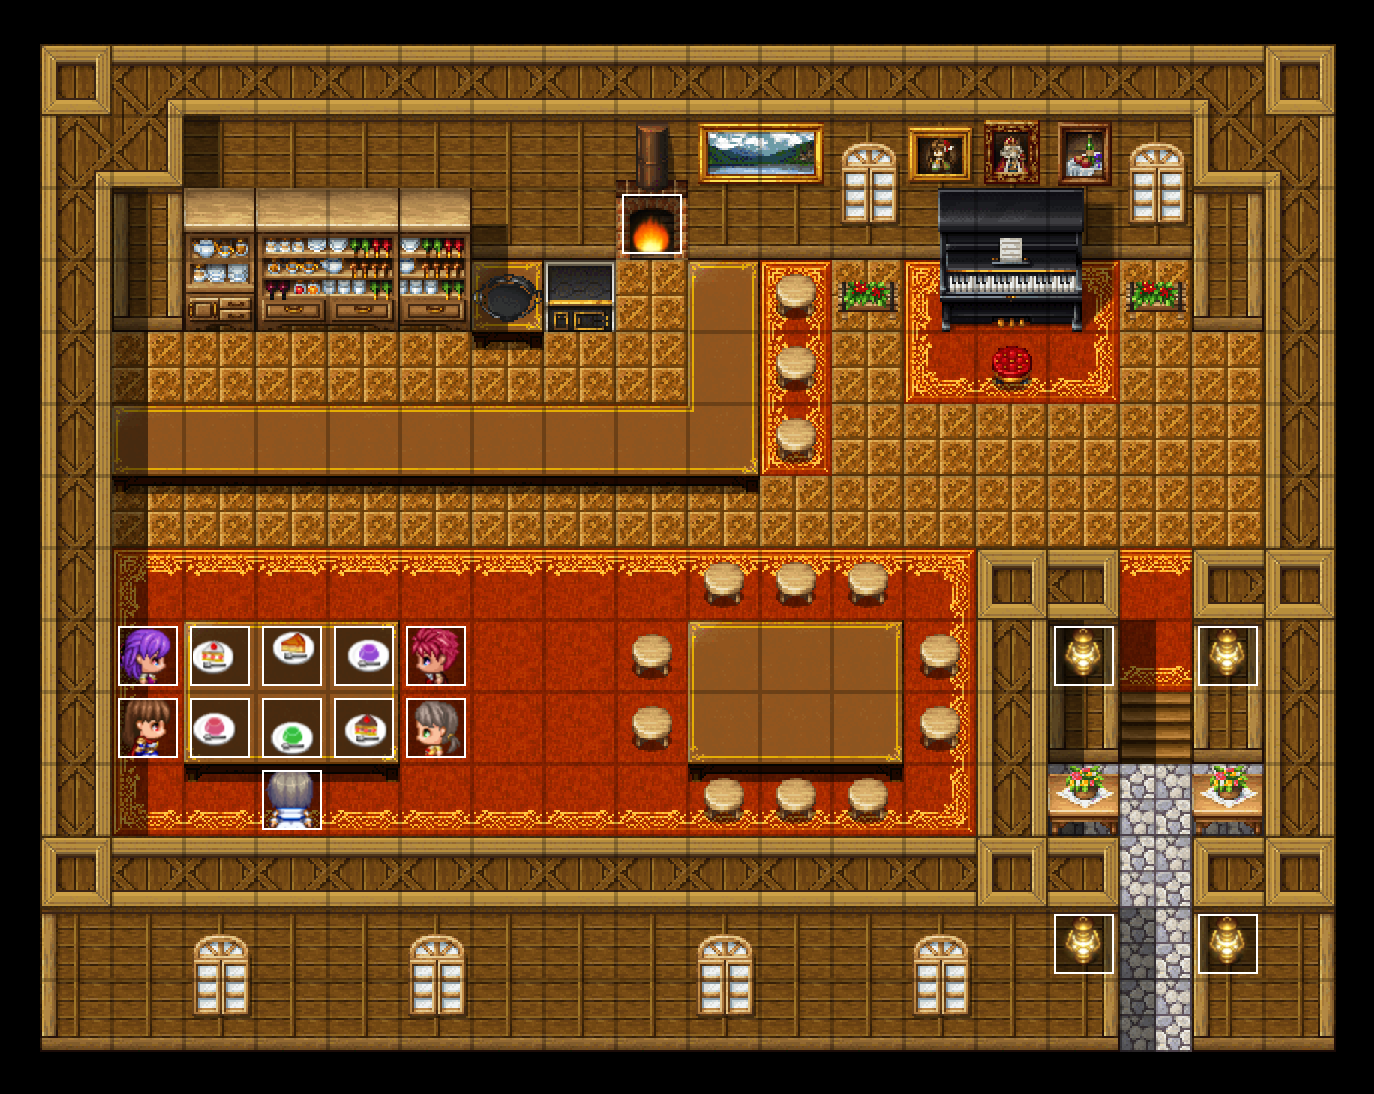
\includegraphics[scale=0.4]{Textuais/Pictures/Lanchonete.png}
		      \fonte{Criado pelo autor.}\label{fig:lanchonete}
	      \end{figure}

	\item Papelaria da Família: Coração da trama, onde muitos dos mistérios e desafios se concentram.

	      \begin{figure}[ht]
		      \centering
		      \caption{Mapa Papelaria.}
		      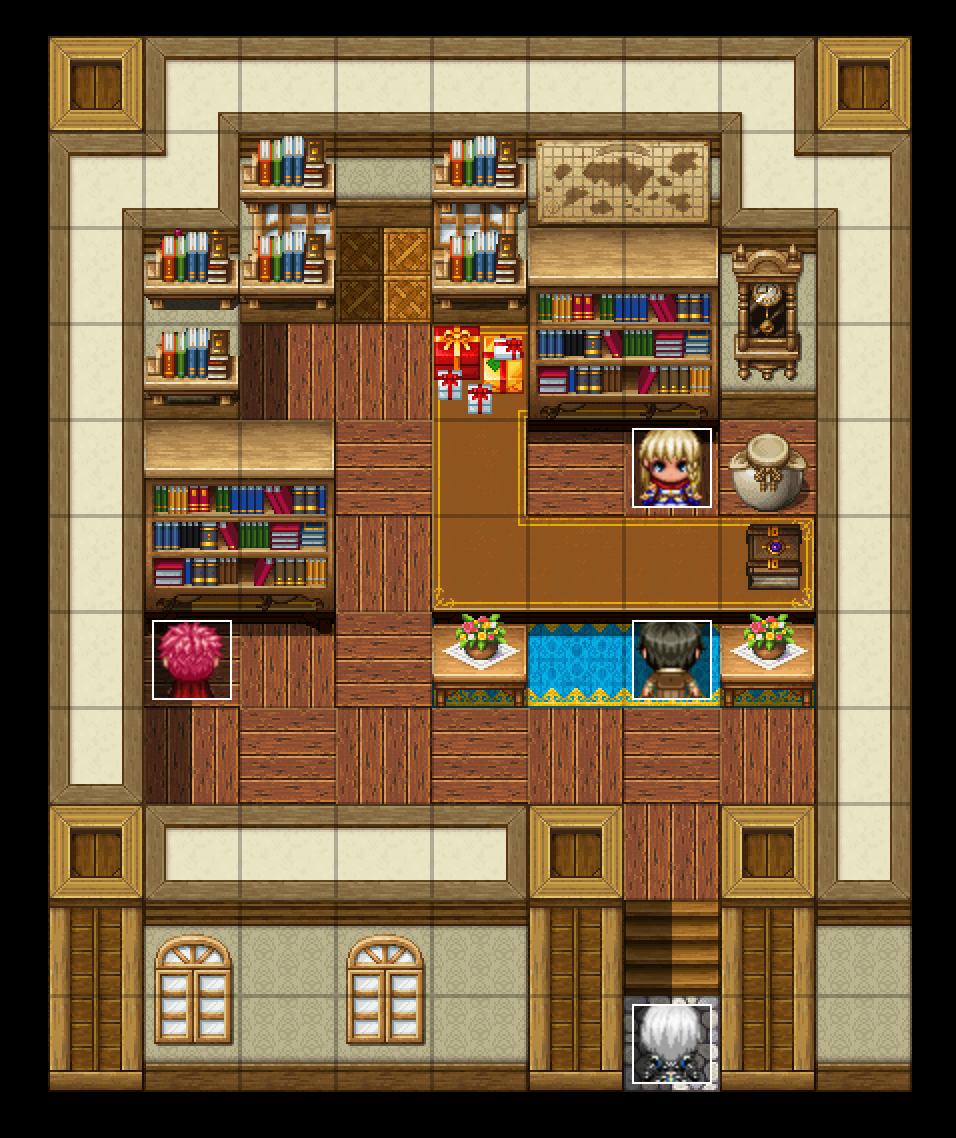
\includegraphics[scale=0.5]{Textuais/Pictures/Papelaria_Familia.png}
		      \fonte{Criado pelo autor.}\label{fig:papelaria-familia}
	      \end{figure}

	\item Cozinha da Papelaria: Local onde Chico encontra o Josimar e faz descobertas, como o problema com a geladeira.

	      \begin{figure}[ht]
		      \centering
		      \caption{Mapa da cozinha da papelaria.}
		      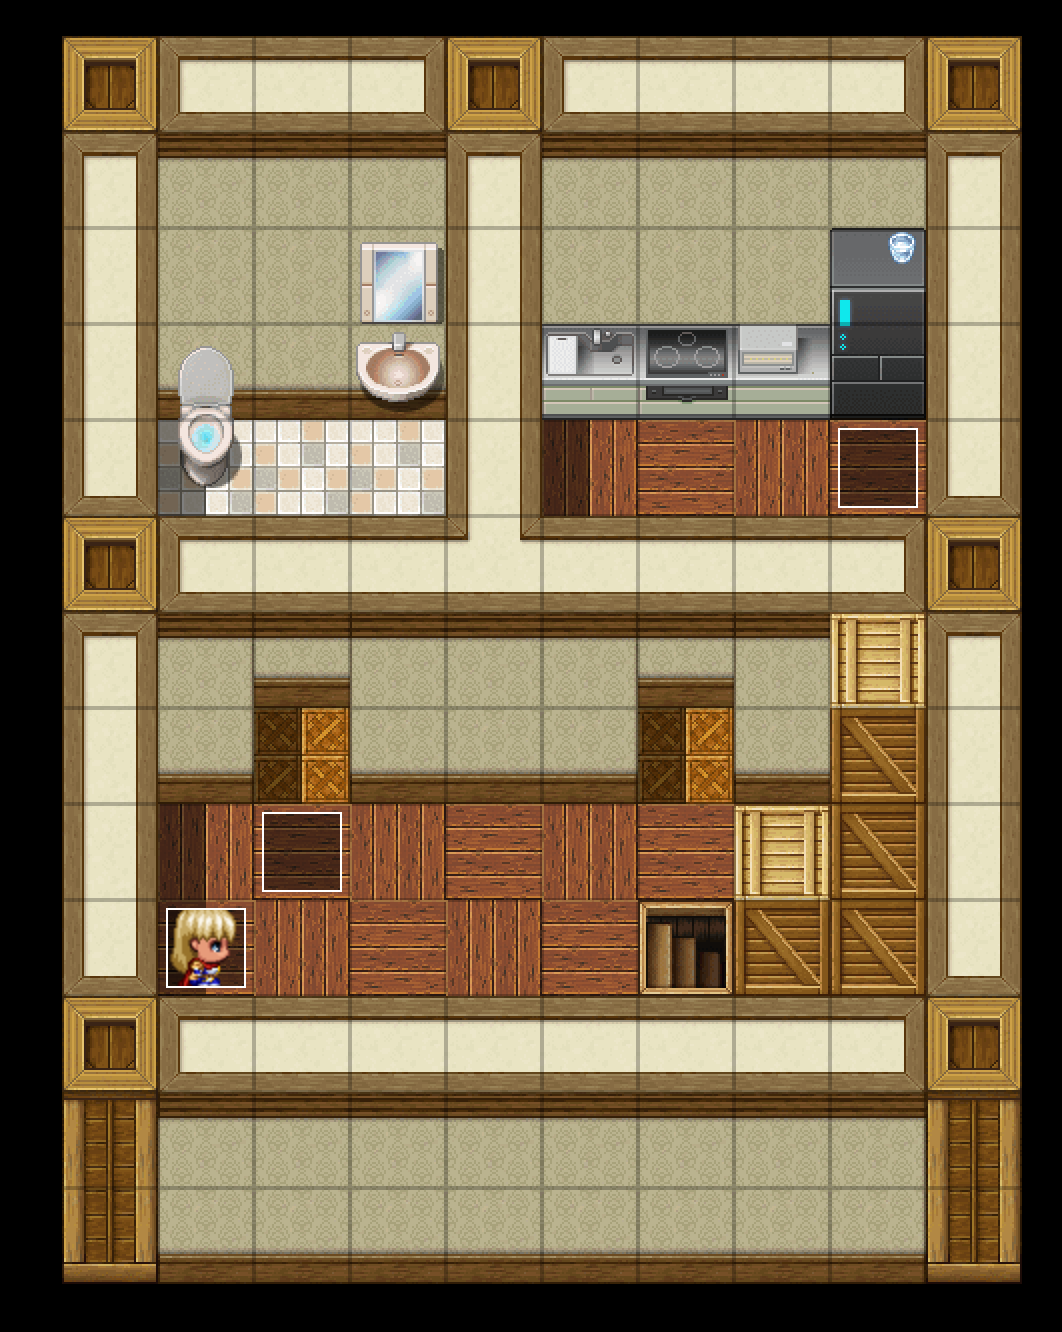
\includegraphics[scale=0.5]{Textuais/Pictures/Cozinha_papelaria.png}
		      \fonte{Criado pelo autor.}\label{fig:lanchonete}
	      \end{figure}

	\item Porão da Papelaria: Ambiente sombrio e cheio de mistérios, onde Chico enfrenta a Ratazana.

	      \begin{figure}[ht]
		      \centering
		      \caption{Mapa do porão da papelaria.}
		      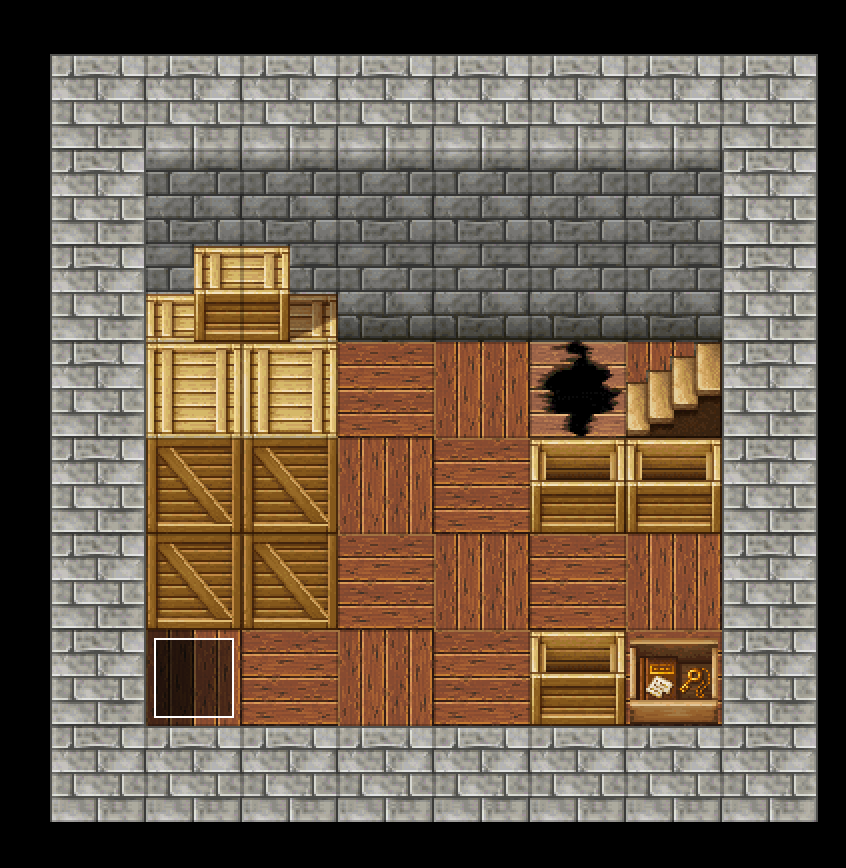
\includegraphics[scale=0.4]{Textuais/Pictures/Porao_papelaria.png}
		      \fonte{Criado pelo autor.}\label{fig:porao-papelaria}
	      \end{figure}

	      \newpage

	\item Hospital: Local de cuidado e recuperação, podendo ser cenário de eventos dramáticos, como o ataque da ratazana.

	      \begin{figure}[ht]
		      \centering
		      \caption{Mapa do hospital.}
		      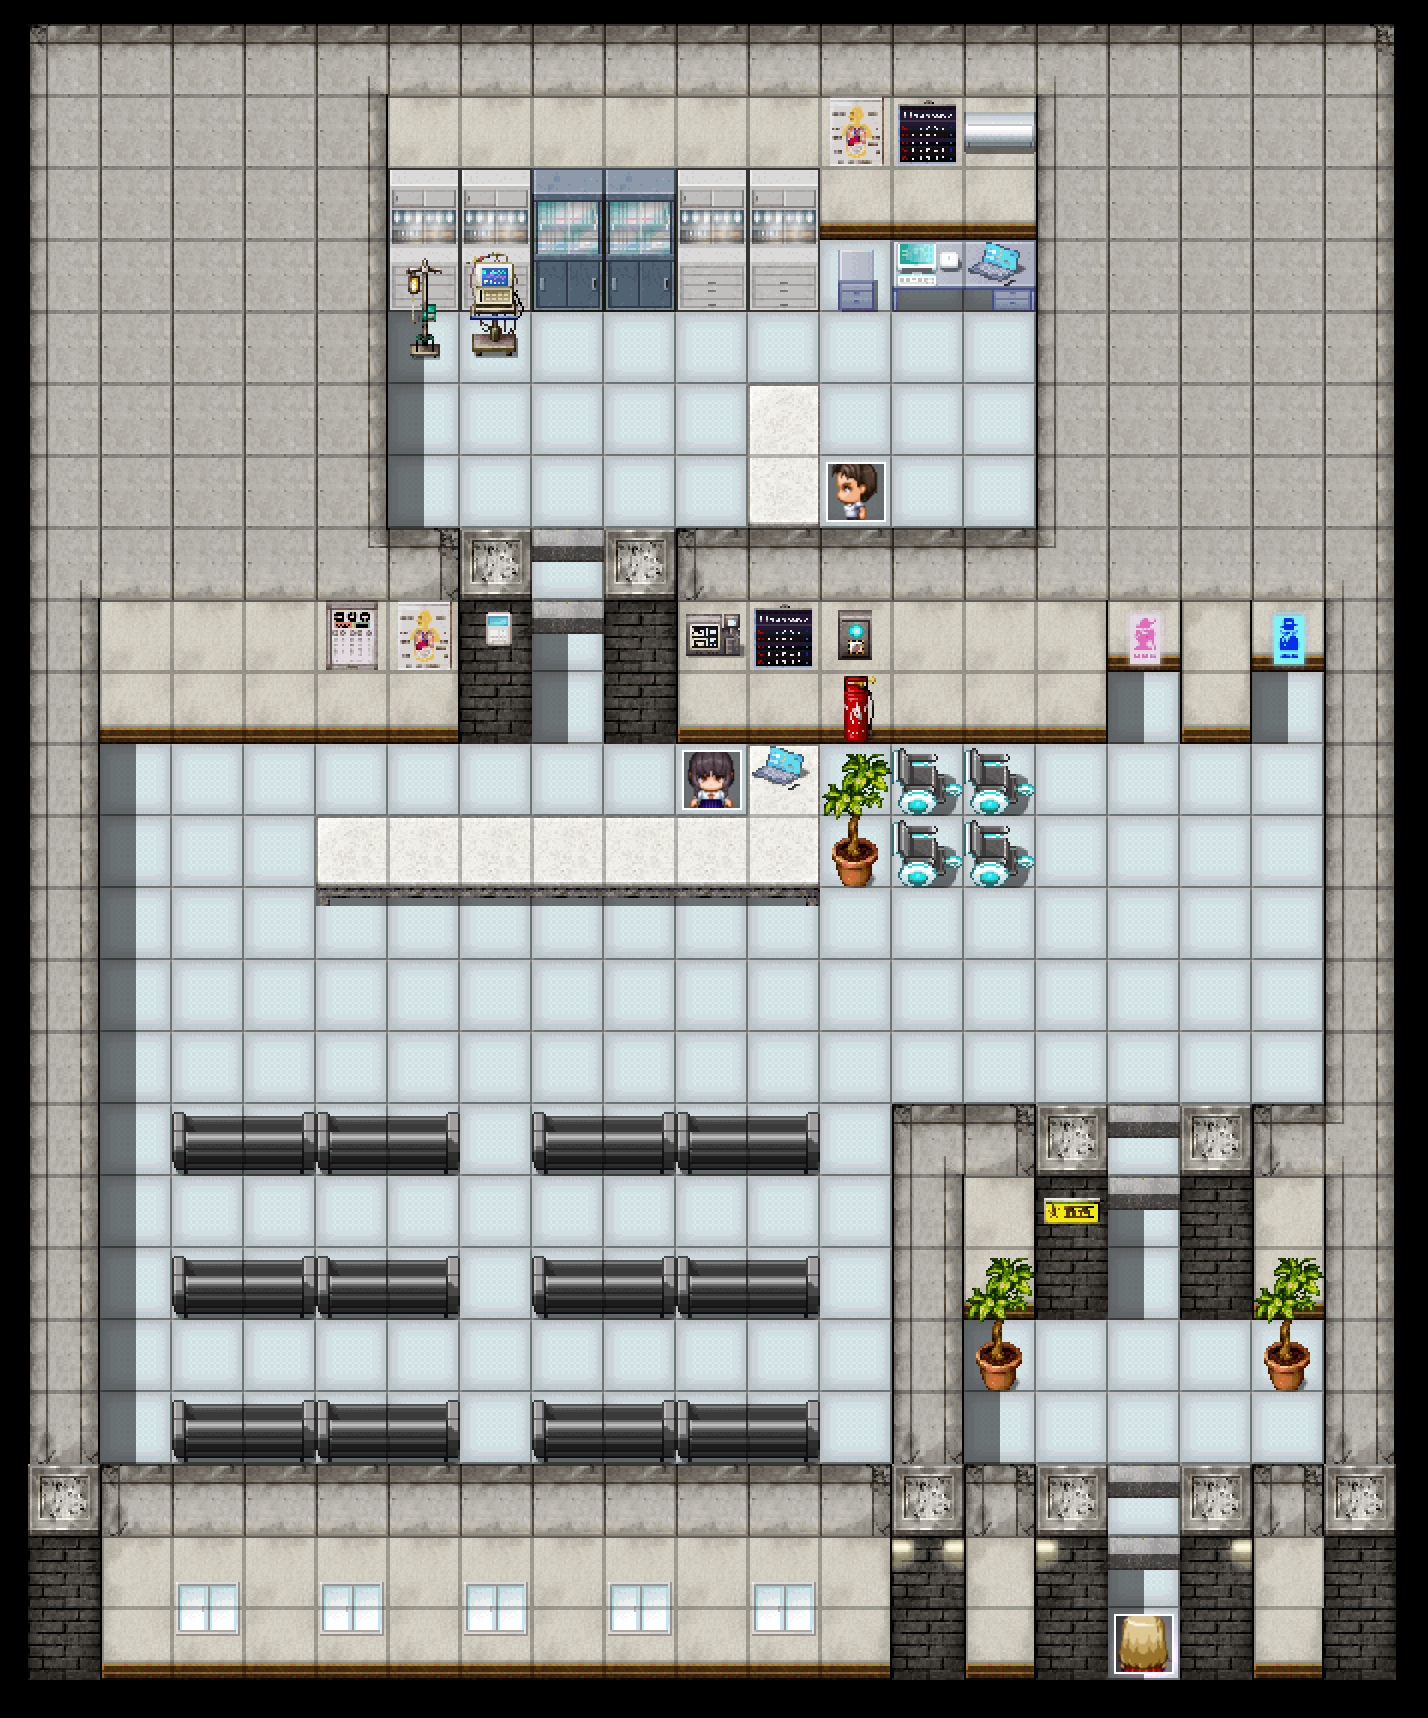
\includegraphics[scale=0.5]{Textuais/Pictures/Hospital.png}
		      \fonte{Criado pelo autor.}\label{fig:hospital}
	      \end{figure}

	      \newpage

	\item Loja de Ferragens: Fornecedora da lanterna para as investigações de Chico.

	      \begin{figure}[ht]
		      \centering
		      \caption{Mapa da loja de ferragens.}
		      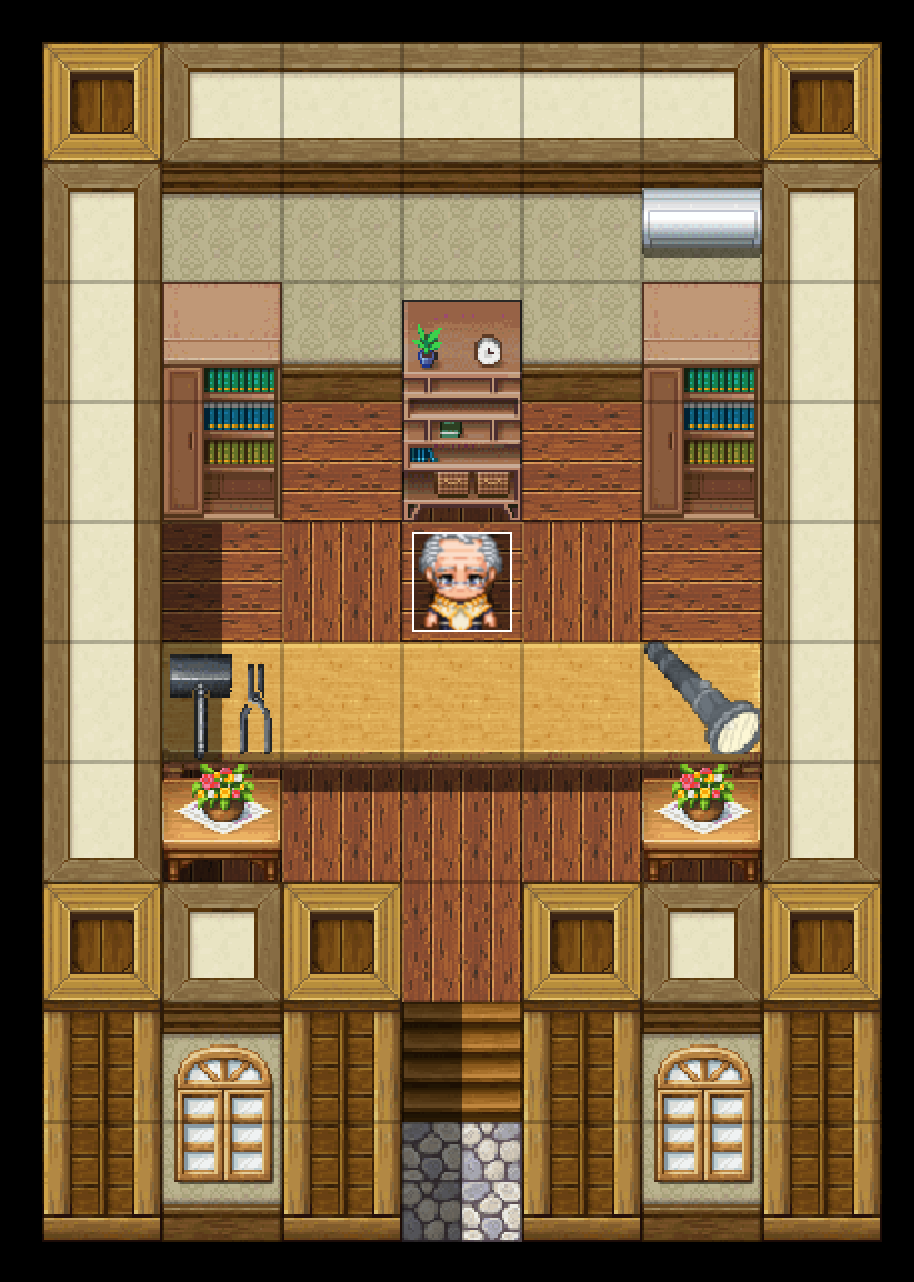
\includegraphics[scale=0.3]{Textuais/Pictures/Loja_Ferragens.png}
		      \fonte{Criado pelo autor.}\label{fig:loja-ferragens}
	      \end{figure}

	\item Casa do Chico: Espaço de união e diálogo da família, proporcionando um contraste com as áreas de mistério e aventura.

	      \begin{figure}[ht]
		      \centering
		      \caption{Mapa da casa do Chico.}
		      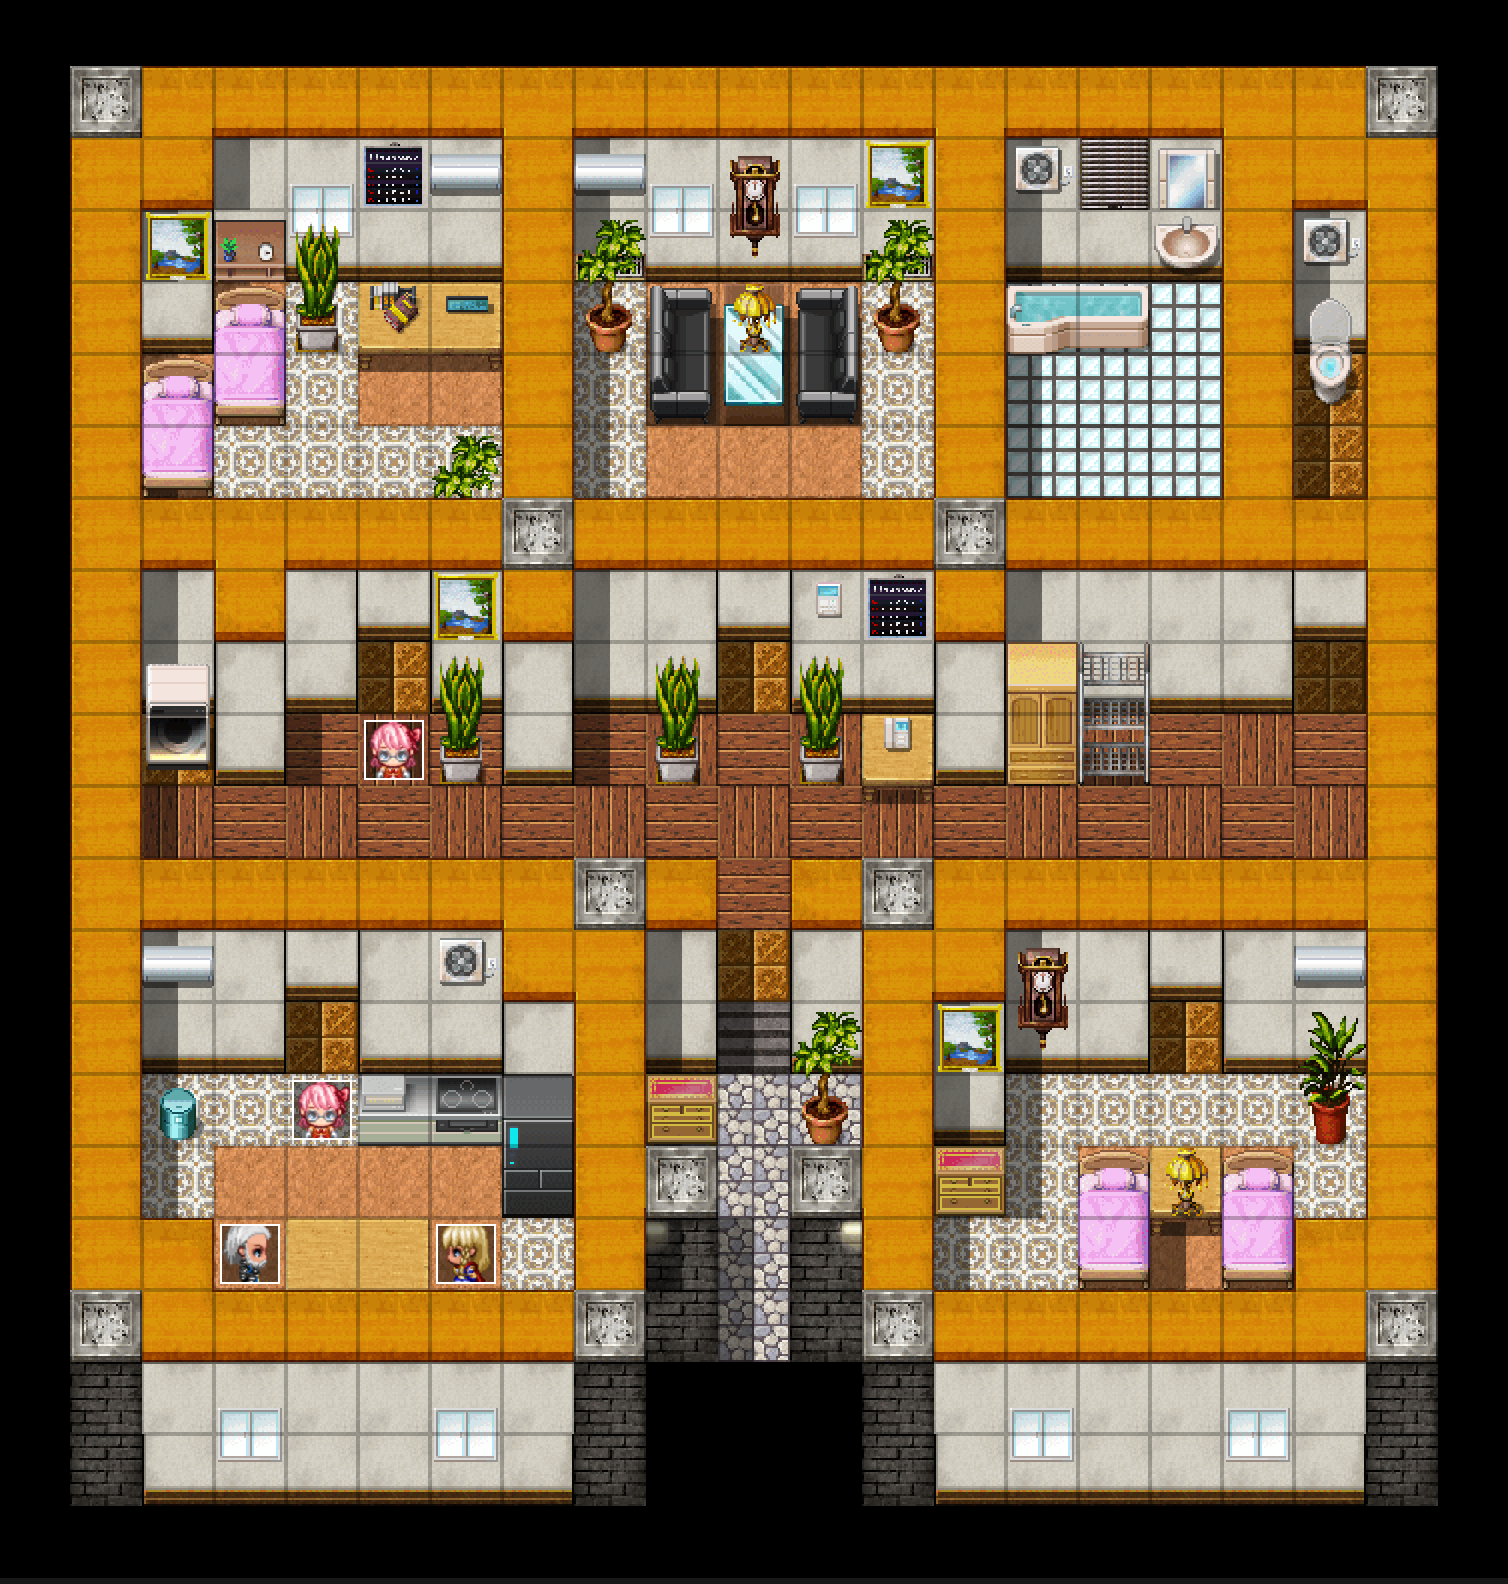
\includegraphics[scale=0.3]{Textuais/Pictures/Casa_chico.png}
		      \fonte{Criado pelo autor.}\label{fig:casa-chico}
	      \end{figure}

\end{itemize}

\chapter{Considerações finais}

Este trabalho buscou abordar a relevância da educação financeira para o público infantil, um tema de grande importância na sociedade contemporânea. Foi desenvolvido um jogo digital educativo intitulado "Mistério Financeiro: A Jornada de Chico", que combina aspectos lúdicos com o ensino de conceitos financeiros básicos. Este jogo foi estruturado com base na narrativa da Estratégia Nacional de Educação Financeira (ENEF), visando proporcionar uma experiência educativa rica e engajadora para crianças do 5º ano do Ensino Fundamental.

O jogo apresenta uma estrutura de RPG interativo, onde as escolhas do jogador influenciam diretamente o andamento da história. O enredo é centrado em Chico, um menino que se depara com desafios financeiros em sua família e decide investigar as causas. As decisões tomadas pelos jogadores ao longo da narrativa não apenas afetam o resultado da história, mas também oferecem oportunidades de aprendizado sobre gestão de recursos, economia e planejamento financeiro.

A experiência de desenvolvimento deste projeto permitiu a integração de práticas pedagógicas com elementos lúdicos, resultando em um recurso didático que pode ser particularmente eficaz no ensino de conceitos financeiros para crianças. Esta abordagem é consistente com a literatura atual, que enfatiza a importância da gamificação na educação e a necessidade de métodos inovadores que engajem os estudantes e complementem os currículos tradicionais.

\section{Desenvolvimentos Futuros}
Embora o jogo "Mistério Financeiro: A Jornada de Chico" represente um passo significativo na direção de uma educação financeira mais engajadora para crianças, há dois desenvolvimentos futuros essenciais que podem expandir e enriquecer ainda mais este projeto:

\subsection{Teste com Estudantes}
A aplicação prática do jogo em um ambiente escolar, com a participação direta de estudantes do Ensino Fundamental, é fundamental para avaliar sua eficácia educacional. Testes em sala de aula permitiriam observar a interação dos alunos com o jogo, avaliar o grau de engajamento, o entendimento dos conceitos financeiros apresentados e a capacidade de aplicar o conhecimento adquirido em situações práticas. Além disso, o feedback dos professores e alunos seria inestimável para refinar o jogo, ajustar dificuldades e garantir que o conteúdo esteja alinhado com os objetivos pedagógicos.

\subsection{Implementação de Outras Histórias da ENEF}
A expansão do jogo com a inclusão de outras narrativas e cenários presentes nos materiais da ENEF enriqueceria o espectro de experiências e aprendizados oferecidos. Essa diversificação permitiria abordar uma gama mais ampla de tópicos financeiros e proporcionar diferentes contextos e desafios aos jogadores. Além disso, ofereceria aos alunos a oportunidade de explorar diversas situações financeiras, cada uma com seus próprios desafios e lições, aumentando a abrangência e a profundidade do aprendizado.

\section{Reflexão Final}
O desenvolvimento de "Mistério Financeiro: A Jornada de Chico" representa um esforço significativo para tornar a educação financeira mais acessível e atraente para o público infantil. O uso de jogos educativos digitais como ferramentas pedagógicas é uma abordagem promissora que pode complementar os métodos de ensino tradicionais, proporcionando um ambiente de aprendizagem mais dinâmico e interativo. A implementação deste projeto e os desenvolvimentos futuros propostos têm o potencial de contribuir significativamente para a formação de jovens mais conscientes e preparados para gerir suas finanças pessoais de forma responsável.

% -----------------------------------------------------------------
% ELEMENTOS PÓS-TEXTUAIS
% -----------------------------------------------------------------
\postextual

% Referências bibliográficas
\bibliography{references}	% Elemento Obrigatório

%% ----------------------------------------------------------
% Glossário
% ----------------------------------------------------------

%Consulte o manual da classe abntex2 para orientações sobre o glossário.

%\glossary




% ----------------------------------------------------------
% Glossário (Formatado Manualmente)
% ----------------------------------------------------------

\chapter*{GLOSSÁRIO}
\addcontentsline{toc}{chapter}{GLOSSÁRIO}

{ \setlength{\parindent}{0pt} % ambiente sem indentação

	\textbf{Ardósia}: Rocha metamórfica sílico-argilosa formada pela transformação da argila sob pressão e temperatura, endurecida em finas lamelas.

	\textbf{Arenito}: rocha sedimentária de origem detrítica formada de grãos agregados por um cimento natural silicoso, calcário ou ferruginoso que comunica ao conjunto em geral qualidades de dureza e compactação.

	\textbf{Feldspato}: grupo de silicatos de sódio, potássio, cálcio ou outros elementos que compreende dois subgrupos, os feldspatos alcalinos e os plagioclásios.






} % fim ambiente sem indentação


				% Elemenuto Opcional
%
% ----------------------------------------------------------
% Apêndices
% ----------------------------------------------------------

% ---
% Inicia os apêndices
% ---
\begin{apendicesenv}

	% Imprime uma página indicando o início dos apêndices
	%\partapendices

	% ----------------------------------------------------------
	\chapter{TÍTULO}
	% ----------------------------------------------------------


\end{apendicesenv}
% ---				% Elemento Opcional
%
% ----------------------------------------------------------
% Anexos
% ----------------------------------------------------------
%
% ---
% Inicia os anexos
% ---
\begin{anexosenv}

	% Imprime uma página indicando o início dos anexos
	%\partanexos

	% ---
	\chapter{TÍTULO}
	% ---



\end{anexosenv}
				% Elemento Opcional
%
%%---------------------------------------------------------------------
%% INDICE REMISSIVO
%%---------------------------------------------------------------------

%\phantompart
%\printindex

%---------------------------------------------------------------------

%%---------------------------------------------------------------------
%% INDICE REMISSIVO (Formatado Manualmente)
%%---------------------------------------------------------------------

\chapter*{ÍNDICE}
\addcontentsline{toc}{chapter}{ÍNDICE}

{ \setlength{\parindent}{0pt}  % ambiente sem indentação

	Andesito, 22, 50, 73

	Argila, 52, 75, 121

	Basalto, 25, 230, 235





} % fim ambiente sem indentação


		% Elemento Opcional

\end{document}

% -----------------------------------------------------------------
% Fim do Documento
% -----------------------------------------------------------------